\documentclass{article}

% Double-blind main-track submission.
\usepackage{manuscript}

\usepackage[utf8]{inputenc}
\usepackage[T1]{fontenc}
\usepackage{hyperref}
\usepackage{url}
\usepackage{booktabs}
\usepackage{amsfonts}
\usepackage{amsmath}
\usepackage{amssymb}
\usepackage{graphicx}
\usepackage{xcolor}
\usepackage{microtype}
\usepackage{multirow}
\usepackage{placeins}  % \FloatBarrier to keep figures with their text

% Loosen LaTeX float placement: allow figures to take more of a page
% and require less text per page so figures don't all defer to the end.
\renewcommand{\topfraction}{0.92}
\renewcommand{\bottomfraction}{0.92}
\renewcommand{\textfraction}{0.05}
\renewcommand{\floatpagefraction}{0.7}
\setcounter{topnumber}{3}
\setcounter{bottomnumber}{2}
\setcounter{totalnumber}{4}

% Visible placeholder macro for numbers pending experiment completion.
% Final submission: audit \TODO and replace each with real values.
\newcommand{\TODO}[1]{\textcolor{red}{\textbf{[TODO: #1]}}}

% Uncertainty-flagging macros (final submission: review whether each \uncertain
% should remain coloured or be promoted to settled black).
% \uncertain{} marks an inline claim as interpretive / not directly tested:
%   the prose still reads naturally, the colour signals "this is reading
%   beyond what the data directly shows".
% \pendnote{} converts a "single-seed / multi-seed left for future work / TODO" caveat
%   into a footnote so the main paragraph reads cleanly.
% \uncertain inlines a hedge in plain black; \pendnote becomes a plain footnote
% (no colour) — submission style choice 2026-05-06.
\newcommand{\uncertain}[1]{#1}
\newcommand{\pendnote}[1]{\footnote{\small #1}}

% \hcpending{} flags claims that depend on incoming high-compute (hc)
% cluster results currently in training; the prose reads naturally and
% the colour signals "this is the predicted/expected reading; concrete
% numbers will replace the placeholder once the result lands". Distinct
% colour from \uncertain (orange) so reviewers can tell apart "interpretive
% beyond data" from "awaiting data".
\definecolor{hcpendingcol}{RGB}{0,128,128}
\newcommand{\hcpending}[1]{{\color{hcpendingcol}#1}}

% \todoblue{} — INTERNAL marker (not for reviewers). Flags analyses /
% experiments that are short-compute (≤1 day analysis-only OR overnight)
% and therefore NOT genuinely "future work" — they are this paper's
% pre-DDL priority queue. Workflow: pick one, run it, replace the
% \todoblue{} block with results in plain black. Anything still flagged
% blue at submission time gets either (a) downgraded to "future work" if
% truly out of time, or (b) inlined-as-result if landed. Distinct colour
% from \uncertain (orange) and \hcpending (teal) so we can grep just the
% blue queue. NOTE: strip these (or convert to plain text) before camera-
% ready / reviewer-facing build.
\definecolor{todobluecol}{RGB}{30,80,200}
\newcommand{\todoblue}[1]{{\color{todobluecol}#1}}

% \toconfirm{} — INTERNAL marker (not for reviewers). Flags specific
% quantitative results (R², SPL, participation ratios, ID estimates,
% cluster centroids, etc.) that come from the OLD pre-unified-retrain
% checkpoints and therefore must be re-computed once the unified-retrain
% probes (probe-1...4) finish converging. Workflow: post-retrain we
% re-probe all 5 ckpts, then sweep \toconfirm{...} sites and replace
% with the converged number in plain black. Any number still flagged
% red at submission time is a known-stale value that we either failed
% to update (panic) or explicitly chose to keep (rare). Pairs with
% \todoblue{} (which queues NEW analyses): \toconfirm tracks UPDATING
% existing analyses; \todoblue tracks NEW ones. Distinct colour
% (red) from \uncertain (orange), \hcpending (teal), \todoblue (blue).
% NOTE: strip / replace before camera-ready.
\definecolor{toconfirmcol}{RGB}{200,30,30}
\newcommand{\toconfirm}[1]{{\color{toconfirmcol}#1}}

\title{Sensor Structure Shapes the Format of \\ Cognitive Maps in Navigation Agents}

\author{%
  Anonymous authors\\
  Paper under double-blind review\\
}

\begin{document}
\maketitle

\begin{abstract}
Visual perception and spatial memory in embodied AI are typically treated as independent modules, but scaling visual encoders often fails to yield robust spatial representations. We investigate whether sensor structure inherently shapes the format of spatial memory. We train a group of RL navigation agents where architecture, task, and training are held strictly fixed, varying only the spatial bandwidth of the visual encoder. We demonstrate that while all agents reach behavioral convergence, their hidden-state position codes fundamentally diverge. Under a vision-limited (bottleneck) encoder, position condenses into a scene-invariant, linearly-readable axis. Under a rich encoder, position information scatters into non-linear, scene-conditional directions. We frame this format shift as an emergent capacity allocation tradeoff between pre-formatted visual features and recurrent temporal integration. Furthermore, causal interventions reveal a strict dissociation between probe-readability and policy reliance, exposing a critical blind spot in correlational interpretability methods. Our findings position sensor visual structure as a fundamental lever on cognitive-map format, generating architecture-agnostic predictions for transformer-based navigators, and suggesting that bandwidth-restricting perception (such as foveation) is actively cognition-enabling rather than merely compute-saving.
% The format of spatial memory in the hippocampus varies with a species' visual ecology, but whether this reflects a general sensor--memory coupling is hard to test directly: animal sensor ecology is fixed within species, and AI systems rarely co-train encoder and memory across a graded sensor design. We test this in silicon: a navigation agent where only the visual sensor varies along an encoder spatial-bandwidth axis, with architecture, task, and training held fixed. Across the axis every agent reliably reaches the goal, yet the hidden-state code for position differs in form: with a vision-limited encoder, position concentrates into a scene-invariant linearly-readable axis; with a rich encoder, it distributes into non-linear directions and is partly carried by encoder features. Linear readability collapses faster than total position information: a format shift, not a total-information collapse. We frame this as an emergent \emph{capacity allocation} between the encoder route and the memory-integration route, read along three complementary views (magnitude, format, consumption). Probe-readable position dissociates from policy reliance in two off-diagonal cases: a bottleneck-encoder agent under-weights its readable code, while a rich-encoder agent reads a scene-history substitute despite no readable code; a complementary causal ablation shows the readable axis is one window into a distributed population code, not its substrate. The work positions sensor structure as a training-time lever on cognitive-map format, generates a falsifiable architecture-agnostic prediction for transformer navigators, and reframes bandwidth-restricting perception as plausibly cognition-enabling rather than only compute-saving. More broadly, a probe and the downstream policy can read different things from the same representation, a gap more naturally surfaced by comparing matched networks than by probing one in isolation.
\end{abstract}


\section{Introduction}

Visual perception and downstream memory are typically treated as independent modules in a sequential pipeline. Under this modular approach, the encoder is developed as a standalone feature extractor, guided by the assumption that scaling the encoder's capacity will provide a richer set of features for the rest of the system. Recent work, however, demonstrates that this ``plug-and-play'' logic is flawed: even when equipped with high-capacity encoders that excel at object recognition, vision--language models (VLMs) consistently fail at tasks requiring an understanding of 3D layouts and relative positioning~\citep{ramakrishnan2025space,yang2024thinkinginspace}. While others argue that we simply need more spatial training data~\citep{chen2024spatialvlm} or different pretraining objectives~\citep{tong2024eyeswideshut,elbanani2024probing3d}, we propose that the issue lies in the isolation of the components, as cognitive neuroscience has long recognised that sensor structure shapes the format of cognitive maps~\citep{wirth2017gaze,rolls2024why,geva2016remapping,fortin2008blind}. By treating perception and memory as a single, co-trained system, we investigate how the architectural structure of the encoder itself constrains what spatial information can be read from memory.

\begin{figure}[t]
\centering
% Paper-level pipeline schematic. Row 1 (architecture): condition-thumbnail
% column -> ResNet-18 -> sensor stack -> 3-layer LSTM -> policy / h_2.
% Row 2 (analysis): three method-finding columns (probes, geometry,
% intervention) read the frozen top-layer hidden state h_2.
\setlength{\abovecaptionskip}{4pt}
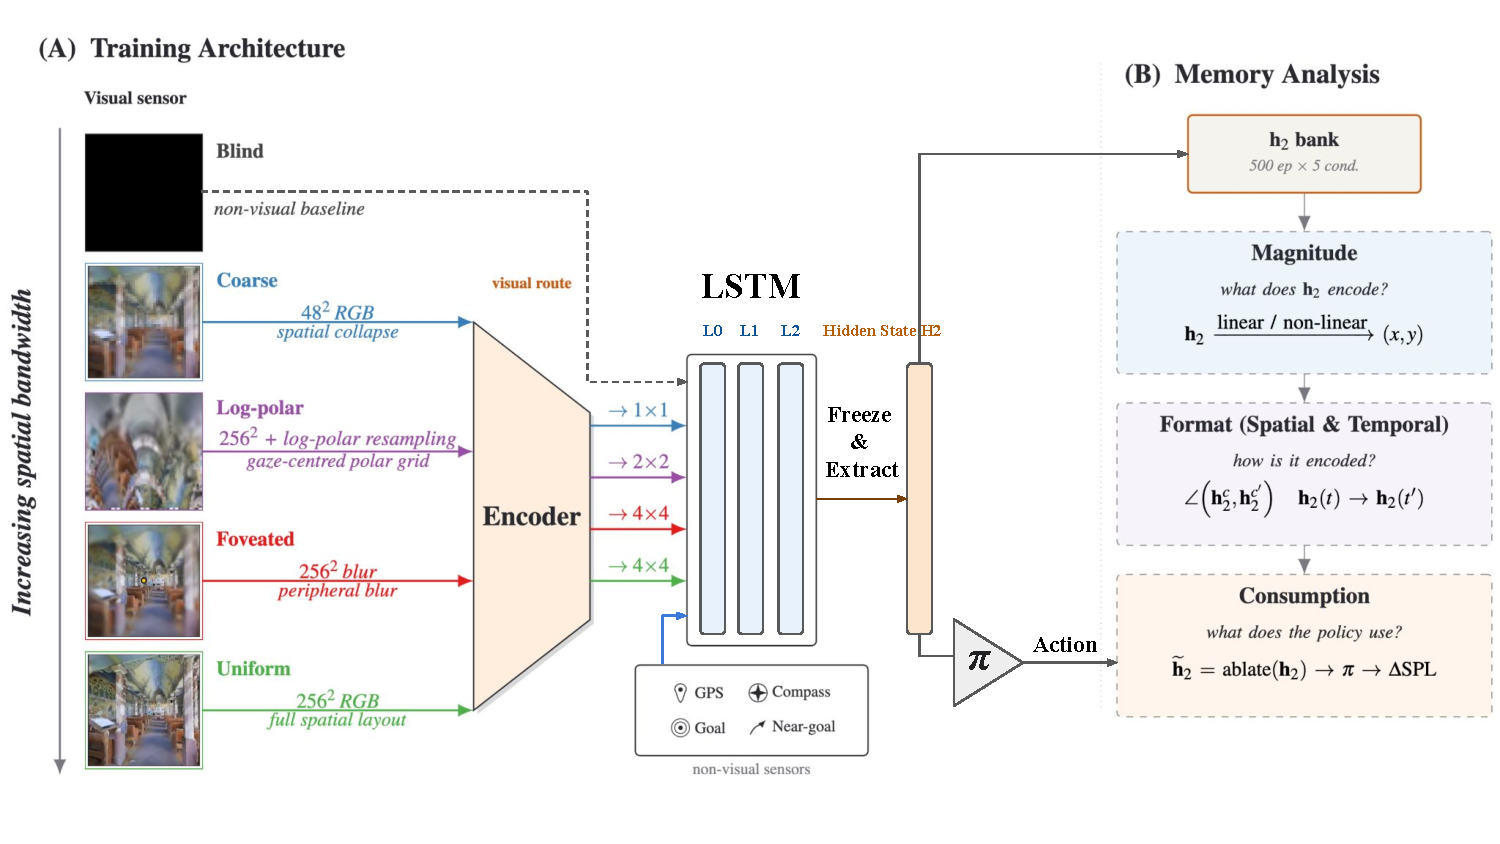
\includegraphics[width=\linewidth]{fig/fig1.pdf}
\caption{\textbf{Experimental setup and analysis pipeline.} \textbf{(A)} Five sensor conditions (leftmost column) ordered by visual bandwidth feed a shared encoder and memory; non-visual sensors enter the memory directly. The top-layer hidden state $\mathbf{h}_2$, which we read as the agent's spatial memory, drives the policy. \textbf{(B)} Read spatial memory along three views: Magnitude (decodability, §\ref{sec:h1}), Format (intrinsic structure, §\ref{sec:format-spatial}--§\ref{sec:tgm}), and Consumption (behavioural intervention, §\ref{sec:dissociation}).}
\label{fig:setup}
\end{figure}

We bridge this gap in a silicon setting. Building on deep-RL navigation agents known to develop cognitive-map-like representations even in the absence of vision~\citep{wijmans2023emergence,banino2018grid,cueva2018grid},\footnote{\small ``Cognitive map'' in our paper is operationalised as the linearly-decodable world-frame position code at the policy-readable hidden state. Aspects of the broader concept~\citep{epstein2017cognitive} are engaged by our LOSO scene-invariance test (relational across rooms) and predictive-horizon analysis (SR-style future-state code, \citealt{stachenfeld2017predictive}); hierarchical scene clustering and topological reachability are deferred to follow-up.} we introduce a comparative testbed that holds the encoder backbone, memory, task, optimisation, and reward entirely fixed, and varies a single degree of freedom: the visual bandwidth of the visual sensor across five conditions (Figure~\ref{fig:setup}).

We hypothesise an emergent \emph{capacity-allocation} principle: the visual encoder and the integration of continuous sensor history (e.g., GPS) compete for a finite hidden-state budget. Our results are consistent with this tradeoff. As visual bandwidth increases, the linearly-readable, world-frame position signal in memory collapses monotonically, even though every agent still reaches the goal. We characterise this reallocation along three complementary views: \emph{magnitude} (how much linearly-accessible position information lives in memory), \emph{format} (which subspace carries it across conditions), and \emph{consumption} (which route the policy actually uses for behaviour). To guard against single-method artefacts, we triangulate findings across multiple probe families and held-out scenes, and ground the format shift behaviourally with asymmetric memory transplants: rich-encoder policies fail to navigate using bottleneck states, suggesting the representational change is intrinsic to the policy's use of memory rather than an artefact of the probing framework~\citep{orozco2025emergentopenvla}.

\noindent Our contributions are three. \textbf{(i)~The capacity-allocation hypothesis.} A candidate framework relating visual bandwidth to spatial-memory format along three complementary views (magnitude, format, consumption). The matched-condition design opens an analytical avenue biology cannot easily realise: the systems-neuroscience toolkit applied to a controlled comparative population rather than a single recording. \textbf{(ii)~Probe-readability dissociates from policy mechanism.} Two off-diagonal cases (a bottleneck-encoder agent under-weighting its own readable position code; a rich-encoder agent reading a scene-history substitute despite no readable code) and a complementary causal ablation jointly show that the linearly-readable axis is one window into a distributed population code, not its substrate. \textbf{(iii)~Predictions for transformer navigators and perception design.} A falsifiable prediction for transformer-based navigators (§\ref{sec:discussion}) and an architecture-side reframing of bandwidth-restricting perception (foveation, log-polar) as plausibly cognition-\emph{enabling} rather than only compute-saving, complementing data-side accounts~\citep{chen2024spatialvlm} of VLM spatial-reasoning failures.

\section{Navigation Agents with Sensors of Varying Visual Bandwidth}
\label{sec:setup}
\label{sec:methods-setup}

\noindent\textbf{Agent configurations}\quad We treat sensor structure as the single degree of freedom (Figure~\ref{fig:setup}A; encoder, memory, sensor stack, training, and reward held identical across conditions). Agents are trained on PointGoal navigation in Habitat~\citep{savva2019habitat} with DD-PPO~\citep{wijmans2020ddppo}. The core architecture is a 3-layer LSTM (512-d) reading from a shared non-visual sensor stack (goal-vector, GPS, compass, prev-action), with a linear policy head that consumes the top-layer hidden state $\mathbf{h}_2$. The bandwidth axis spans two regimes at its endpoints: a \emph{bottleneck regime} (blind, coarse) where the encoder is bypassed or cannot resolve spatial features; and a \emph{rich-encoder regime} (foveated, uniform) where the encoder supplies position-correlated visual features per step. Log-polar is added as a control: log-polar resampling (mirroring the log-radial sampling of primate V1 cortical magnification~\citep{schwartz1977spatial}) preserves per-step feature variety while collapsing the encoder feature map, letting us partially disentangle encoder spatial-output dimensionality from per-step feature variety.

\noindent\textbf{Experimental setup}\quad Each agent is trained from scratch for 250M frames on a merged pool of Gibson 0+~\citep{xia2018gibson} (411 scenes) and Matterport3D-train~\citep{chang2017matterport3d} (61 scenes); following standard practice in comparative-cognition modelling~\citep{wijmans2023emergence,banino2018grid,cueva2018grid,schaeffer2023grid}, we use a single training seed per condition. After training, weights are frozen and per-step $\mathbf{h}_2 \in \mathbb{R}^{512}$ is collected from $n{=}500$ deterministic-rollout episodes per condition on the same scene pool (new (start, goal) pairs sampled fresh, not seen during training). The default decoder is a Ridge linear probe ($\alpha{=}10$, 5-fold episode-level cross-validation, with Hewitt--Liang permutation control~\citep{hewitt2019control}). The linear $R^2$ for decoding GPS position from $\mathbf{h}_2$ serves as a proxy for how directly the policy's linear readout can access world-frame position from memory.


\noindent\textbf{Memory divergence under convergent task performance}\quad Despite different visual inputs, all five agents reliably reach the goal (Table~\ref{tab:summary}; $76$--$99\%$ Success, SPL $0.43$--$0.88$), with blind less path-efficient than the four sighted as expected of vision-free integration~\citep{wijmans2023emergence}. To examine how the encoder--memory--policy stack handles this input variation internally, we read $\mathbf{h}_2$ along three views: magnitude (how much linearly-readable position lives in $\mathbf{h}_2$, §\ref{sec:h1}); format (the shape it takes spatially and temporally, §\ref{sec:format-spatial}--§\ref{sec:tgm}); and consumption (which information the policy actually uses under causal intervention, §\ref{sec:dissociation}).

\begin{table}[!t]
\centering
\small
\setlength{\tabcolsep}{6pt}
\caption{\textbf{Navigation performance and spatial probes.} Per condition: SPL, success rate, and mean episode length ($n{=}200$ deterministic-rollout episodes, mean $\pm$ SEM); Ridge probe $R^2$ for decoding GPS position from $\mathbf{h}_2$ at linear and 2-layer-MLP probe depths (5-fold episode-level CV mean $\pm$ std).}
\label{tab:summary}
\begin{tabular}{lcccccc}
\toprule
& & & & \multicolumn{2}{c}{GPS $R^2$} \\
\cmidrule(lr){5-6}
Condition & SPL & Success & Steps & linear & MLP-2 \\
\midrule
Blind                 & $0.43{\pm}0.02$           & $0.76$          & $416{\pm}34$ & $+0.93{\pm}0.04$  & $+0.98{\pm}0.00$ \\
Coarse                & $0.81{\pm}0.02$           & $0.97$          & $154{\pm}19$ & $+0.58{\pm}0.10$  & $+0.75{\pm}0.09$ \\
Foveated              & $0.88{\pm}0.02$           & $0.97$          & $141{\pm}21$ & $+0.18{\pm}0.66$  & $+0.79{\pm}0.05$ \\
Log-polar     & $0.86{\pm}0.01$           & $0.99$          & $124{\pm}15$ & $-0.03{\pm}0.76$  & $+0.63{\pm}0.17$ \\
Uniform               & $0.87{\pm}0.02$           & $0.98$          & $127{\pm}18$ & $-1.79{\pm}2.99$  & $+0.35{\pm}0.80$ \\
\bottomrule
\end{tabular}
\end{table}

\section{Magnitude: Linear Position Code Weakens with Encoder Bandwidth}
\label{sec:h1}
\label{sec:magnitude}

We hypothesise that the agent can localise via two routes: integrating the GPS-sensor stream over time, or reading a position-correlated feature directly off the encoder. The policy's readout from $\mathbf{h}_2$ is linear, so what a linear probe at $\mathbf{h}_2$ recovers is what the policy can use. Across the bandwidth axis, linear GPS $R^2$ declines monotonically from $+0.93$ in blind to $-1.79$ in uniform (Figure~\ref{fig:magnitude}a, Table~\ref{tab:summary}) while every agent still reliably reaches the goal, a representational dissociation rather than a skill gap. A low $R^2$ is consistent with three interpretations: position is absent from $\mathbf{h}_2$, distributed non-linearly (§\ref{sec:format-spatial}), or replaced by another feature the policy reads (§\ref{sec:dissociation}).

\noindent Before any of those readings, two artefactual explanations need ruling out. (i) Linear probes might just be failing on rich-encoder $\mathbf{h}_2$. They are not: the same linear decoder reads distance-to-goal at $R^2 \geq 0.88$ in every condition (Appendix~\ref{app:alt-accounts}); the probe has the capacity, so rich-encoder $\mathbf{h}_2$ simply does not carry world-frame position as a linear target. (ii) The bottleneck--rich split might just track encoder output dimensionality. It does not: log-polar's $\sim 2{\times}2$ feature map sits close to coarse's $1{\times}1$ in raw cell count, yet lands with foveated and uniform on every magnitude diagnostic (Appendix~\ref{app:scaling}). The relevant variable is per-step feature variety, not encoder geometry.

\noindent With the route-shift reading secured, the next question is when in training the allocation appears. Across training (Figure~\ref{fig:magnitude}b), all sighted conditions begin at high linear readability (encoder weights are still random, so memory falls back on integration). The split appears as the encoder becomes informative: rich-encoder conditions decay as they transfer position from memory to the visual route, while coarse's $1{\times}1$ output cannot carry a position code so its memory plateaus, and blind has no encoder route at all so its memory stays stable. The substitution begins around or after task convergence (${\sim}100$M frames for sighted), consistent with a later refinement of an already-working policy rather than co-emerging with skill.

\noindent Where in the LSTM the allocation appears (Figure~\ref{fig:magnitude}c): GPS $R^2$ at the LSTM input $L_0$ is uniformly ${\sim}0.95$ across conditions: the GPS sensor enters memory intact regardless of vision. $L_1$ is dim everywhere; the bandwidth-graded split emerges only at $L_2$, the policy-readable layer. The decline in linear decodability is therefore not a failure of sensor integration, but a specific property of the final, policy-accessible representation.

\noindent Three independent readings converge: bandwidth-graded magnitude (Fig.~\ref{fig:magnitude}a), training-time emergence after task convergence (b), and layer-localised divergence at $L_2$ (c). The encoder's bandwidth tilts a finite-capacity memory from the integration route toward the visual route, and the divergence shows up specifically where the policy reads. Two further unit-level diagnostics (peaked-unit content and a mid-episode random-action perturbation) converge on the same partition (Appendix~\ref{app:magnitude-detail}). However, whether the missing linear position is fundamentally discarded, non-linearly redistributed, or substituted by another feature still stays an open question. Sections \ref{sec:format-spatial} and \ref{sec:dissociation} resolve the critical mechanistic question left open by §\ref{sec:h1}.

\begin{figure}[!t]
\centering
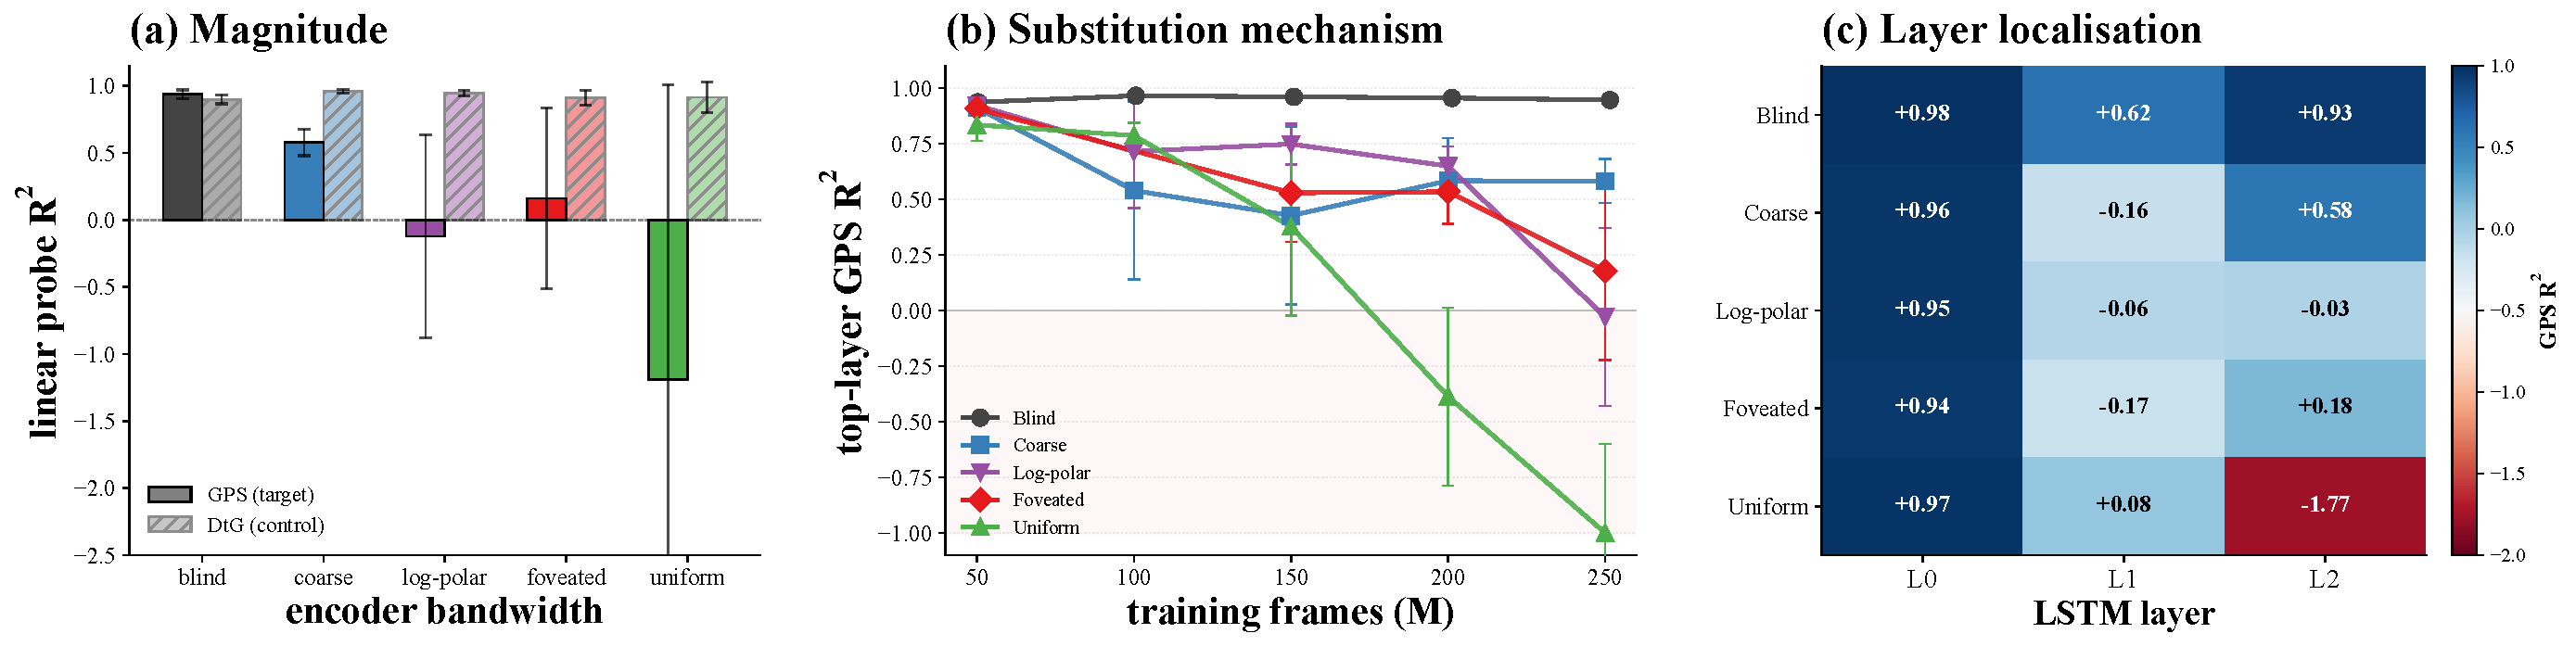
\includegraphics[width=\linewidth]{fig/fig2_magnitude.pdf}
\caption{\textbf{Memory magnitude.} \emph{(a)} Per condition, paired bars give linear probe $R^2$ for GPS (filled) and distance-to-goal (hatched, control). Dashed line at $R^2{=}0$: predict-mean baseline. \emph{(b)} Top-layer GPS $R^2$ at five training snapshots. \emph{(c)} GPS $R^2$ along the LSTM stack ($L_0$ input $\to L_2$ top, same 5-fold CV protocol as (a, b)).}
\label{fig:magnitude}
\end{figure}


\section{Format: Position is Encoded in Distinct Forms Across Conditions}
\label{sec:format}

\subsection{Spatial Format: Collapsed Linear Readability is a Format Shift, not An Information Loss}
\label{sec:format-spatial}
\label{sec:h3-scene-invariance}
\label{sec:h2}

The magnitude collapse of §\ref{sec:h1} does not destroy position information. Non-linear readouts of $\mathbf{h}_2$ recover position where the linear probe fails, and information-theoretic estimates of how much position is encoded shift far less across conditions than the linear $R^2$ does: the collapse is a format shift, not an information loss. The encoder rearranges position along three axes (manifold geometry, scene-invariance, subspace identity) whose boundaries do not coincide.

\begin{figure}[!t]
\centering
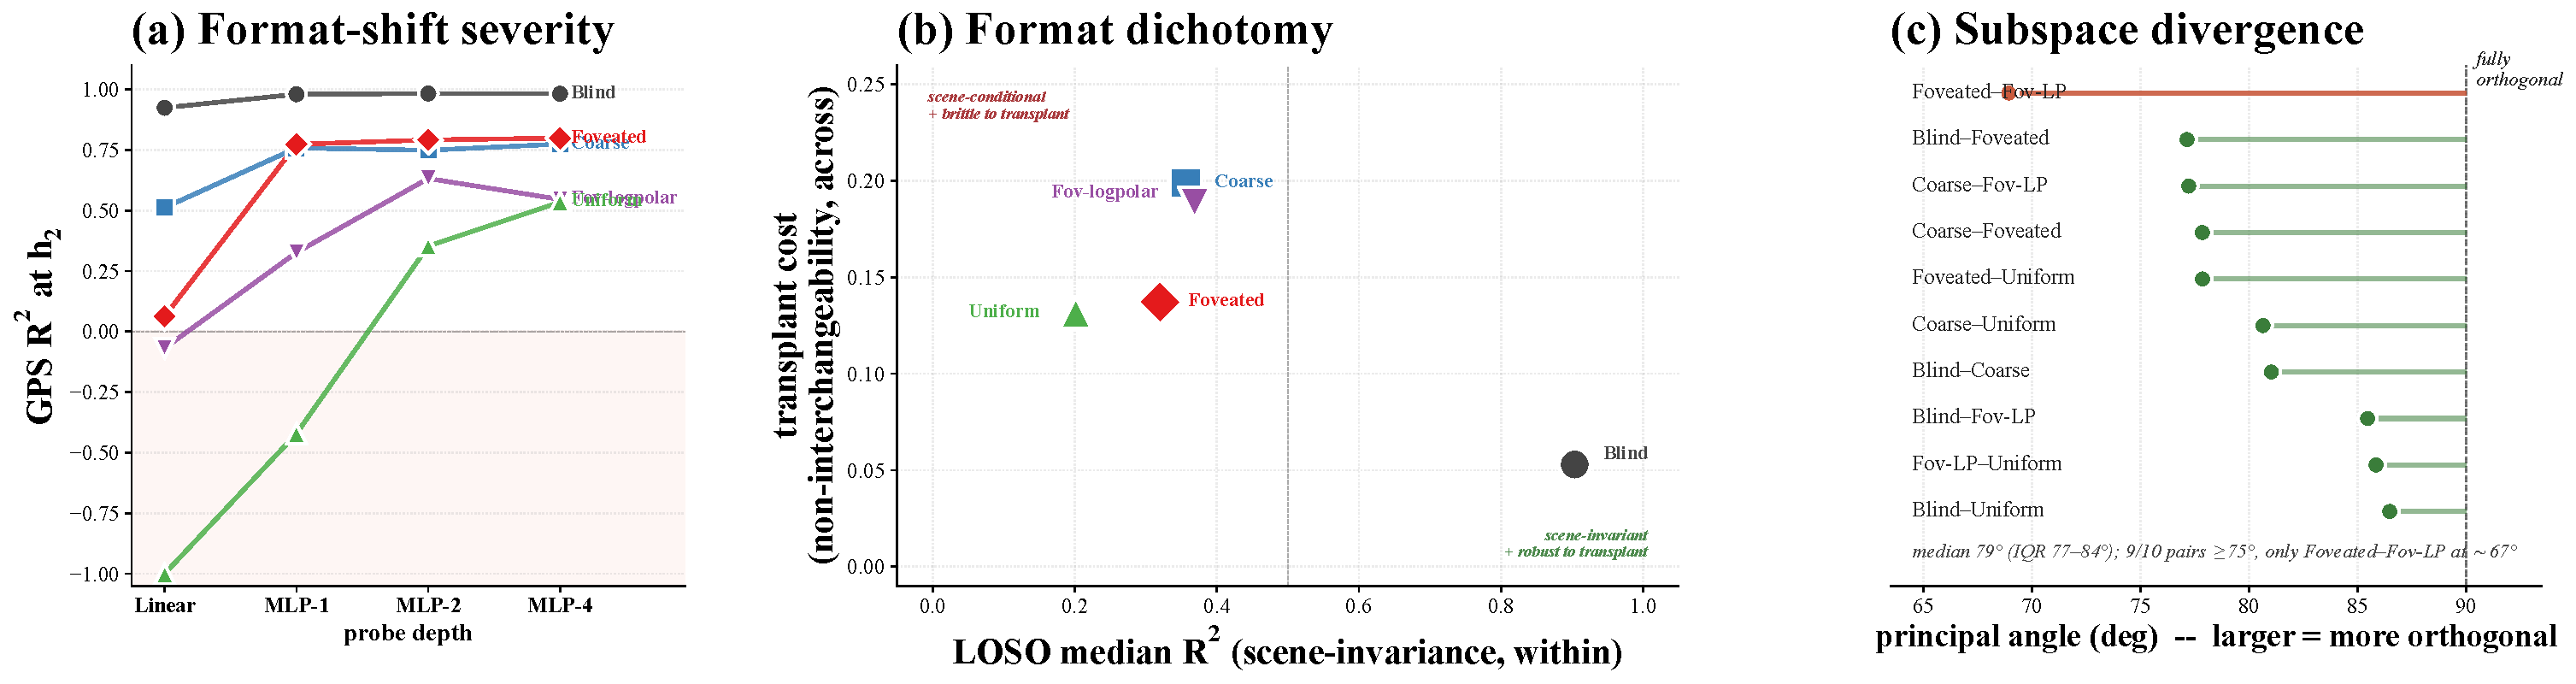
\includegraphics[width=\linewidth]{fig/fig3_format_axis.pdf}
\caption{\textbf{Memory spatial format.} \emph{(a)} PCA-2D projection of top-layer $\mathbf{h}_2$ per condition (1500 random steps each), coloured by ground-truth $x$-coordinate. \emph{(b)} LOSO median $R^2$ for single-axis transfer across rooms vs.\ cross-condition memory-transplant cost. \emph{(c)} Principal angle between every pair of conditions' position-direction subspaces (sorted, with the within-foveated outlier highlighted).}
\label{fig:format_axis}
\end{figure}

The format shift is directly visible in the manifold geometry. A 2D PCA of top-layer hidden states coloured by ground-truth $x$-coordinate (Figure~\ref{fig:format_axis}a) shows blind organising into a single position-graded manifold; coarse is similar but more diffuse; the three rich-encoder conditions fragment into multiple disjoint clouds, each roughly a scene. Inside each cloud the colour gradient is intact, and a 2-layer MLP recovers position at $R^2 \geq 0.35$ even for uniform (Table~\ref{tab:summary}): the cross-scene linear axis a global probe would need has been replaced by scene-conditional gating.

Scene-invariance follows a strict binary split. We test whether a single spatial axis transfers across held-out rooms (LOSO) and whether one condition's memory can drive another's policy (cross-condition transplant cost; Figure~\ref{fig:format_axis}b). Blind uniquely occupies the scene-invariant and transplant-robust quadrant ($\text{LOSO}\,R^2 \approx 0.85$, transplant cost $\approx 0.05$). Any visual input, even the heavily bottlenecked coarse, pushes memory into the scene-conditional and transplant-brittle space. The split sits at the zero-vs-nonzero encoder-bandwidth line, not at low-vs-high: scene-invariance is binary on vision even while magnitude grades continuously.

Subspace identity diverges across all five conditions. Principal angles between position-direction subspaces (Figure~\ref{fig:format_axis}c) place 9 of 10 cross-condition pairs at $\geq 75°$; only the two foveated variants, which share the foveated retina, sit closer at $\sim 67°$: the five position codes are otherwise nearly orthogonal. Rather than converging on rotated, Procrustes-equivalent variants of a single shared map, identical architectures under different sensors settle into nearly orthogonal memory structures. Sensor structure does not merely modulate a common cognitive map; it appears to select among categorically different ones, with each condition's $\mathbf{h}_2$ encoded in a format specific to its own policy.

The three boundaries do not coincide, and that is the structural finding: manifold organisation grades from unified (blind) through diffuse (coarse) to fragmented (rich-encoder); scene-invariance flips binary at vision-on/off; subspaces are condition-specific. Visual bandwidth is therefore a multi-dimensional format lever, not a single knob. This recasts §\ref{sec:h1}'s magnitude collapse: rich-encoder conditions hold position in scene-conditional, non-linear directions, so the global linear probe sees nothing even though the information is still there. Mutual-information estimates of $I(\mathbf{h}_2; \mathrm{pos})$ corroborate the preserved-content reading: total position content stays within a factor of ${\sim}1.3$ across conditions even as linear $R^2$ collapses by orders of magnitude (Appendix~\ref{app:mine}). The blind-vs-sighted dichotomy parallels the no-remapping vs.\ global-remapping spectrum of hippocampal coding under hidden-state inference~\citep{sanders2020remapping}. Biologically, this predicts that blind animals rely on a fundamentally different memory format, not a lower-fidelity version of a sighted map.

\subsection{Temporal Format: Constructed vs Pre-Built Map}
\label{sec:tgm}

\begin{figure}[!t]
\centering
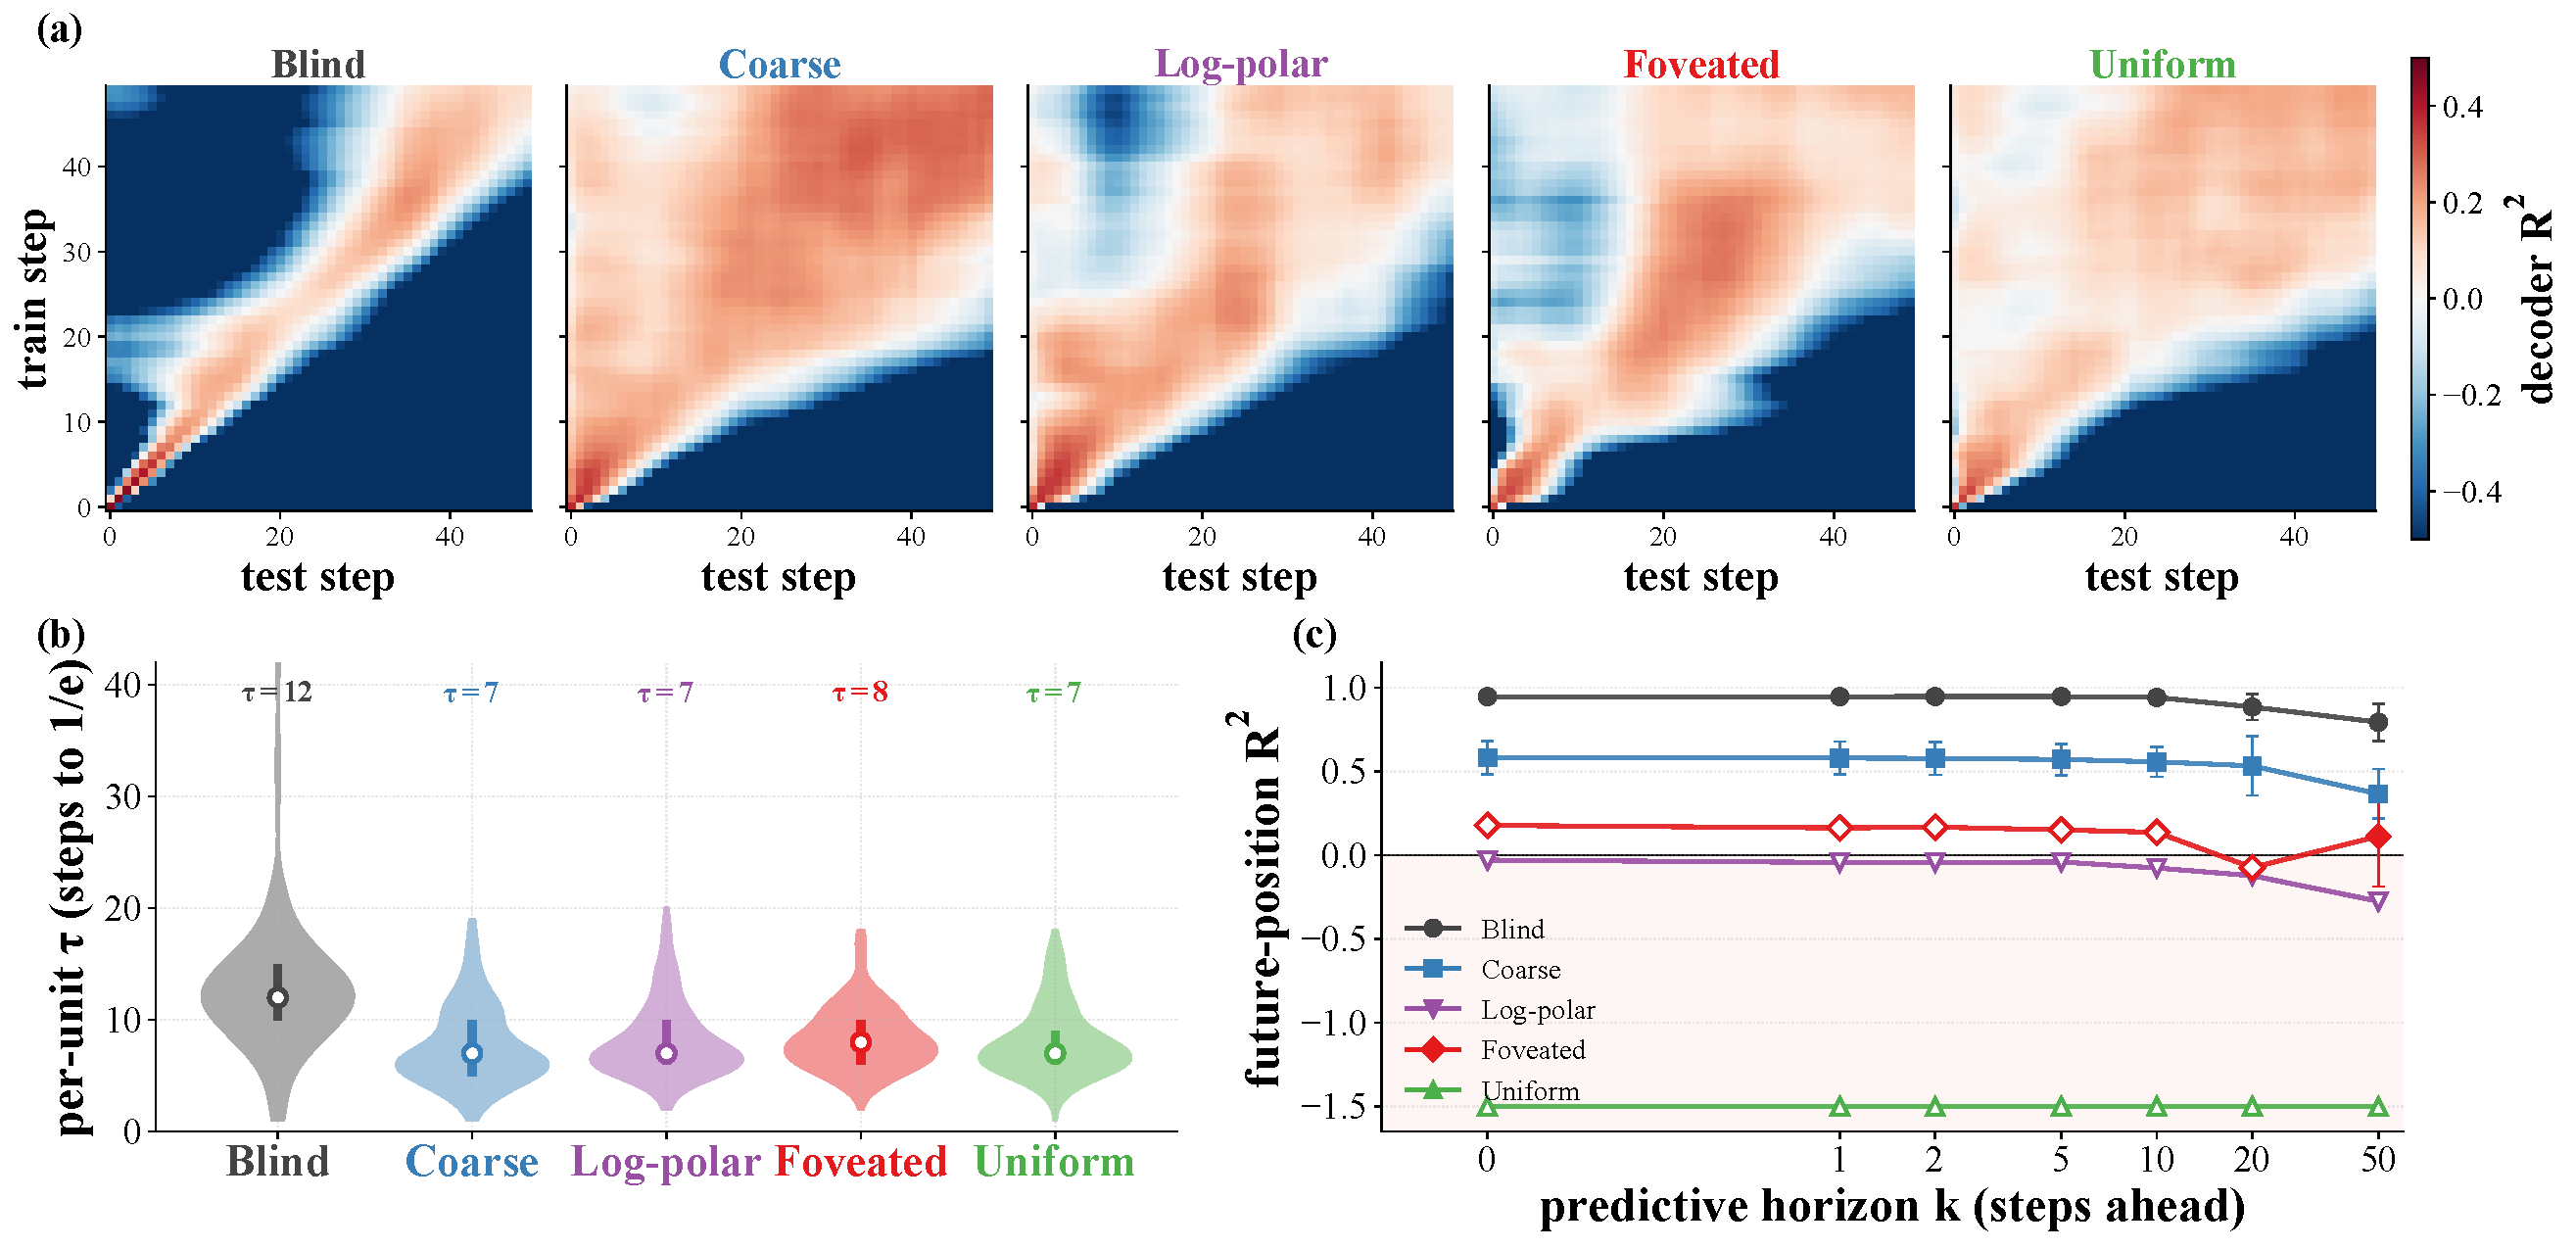
\includegraphics[width=\linewidth]{fig/fig4_temporal.pdf}
\caption{\textbf{Memory temporal format.} \emph{(a) Is the readout axis stationary or does it rotate?} A linear decoder of egocentric goal-vector (offset from agent to goal) trained at one trajectory step and tested at every other step. A square block indicates a stationary readout (coarse); a diagonal stripe indicates a step-by-step rotating one (blind). \emph{(b) How long does a memory unit hold onto its past?} Distribution of per-unit intrinsic timescale $\tau$ across units, defined as the within-episode lag at which the unit's autocorrelation falls to $1/e$. \emph{(c) Does memory carry a forward-rolling trajectory?} $R^2$ of decoding position $k$ steps ahead from current memory; shaded band: $R^2 < 0$.}
\label{fig:temporal_format}
\label{fig:tgm}
\label{fig:cogneuro_battery}
\end{figure}

Beyond spatial format, visual bandwidth changes how memory operates over time. Vision lets the agent anchor its position in a fixed external frame; without vision, position has to be continuously computed from self-motion, and the internal spatial code updates with every step. Blind sits at the active end, sighted at the stable; within sighted, less encoder bandwidth stiffens the readout. The point is not that blind has a cognitive map (Wijmans~\citep{wijmans2023emergence} showed it does), but that an integrated motion-based map and a stable vision-based map are categorically different computational objects, not lower-fidelity versions of one shared representation.

\noindent To distinguish the two regimes we ask a simple question: \emph{is the memory's readout axis stable across the episode, or does it rotate with each step?} The natural readout to test is the egocentric goal-vector (the relative offset from the agent's current position to its goal, expressed in the agent's own reference frame), because that is the spatial quantity the policy must consume to navigate. A linear decoder of this goal-vector, trained at trajectory step $t_{\text{train}}$ and tested at every other step $t_{\text{test}}$~\citep{king2014temporal}, answers the question directly. A stable, world-anchored map yields a square block in the $(t_{\text{train}}, t_{\text{test}})$ heatmap (a single decoder transfers across all steps); a step-by-step constructed map yields a diagonal stripe (the decoder works only near the step it was trained at). Blind shows the diagonal; coarse the largest block; log-polar, foveated, and uniform graded between (Figure~\ref{fig:temporal_format}a). A constructed map cannot be stationary because the construction process is the rotation.

\noindent Beyond what the heatmap reveals about the readout axis, we ask a more basic dynamical question: \emph{how long does a memory unit hold onto its past activity before decorrelating?} This is the \emph{intrinsic timescale}, a property that separates slow-integrating systems from fast-responding ones. We measure it per unit as the autocorrelation of $\mathbf{h}_2$ over within-episode steps and read $\tau$ as the lag at which the autocorrelation crosses $1/e$~\citep{murray2014timescales}; Figure~\ref{fig:temporal_format}b shows the distribution of $\tau$ across units per condition. Blind has a wide, tall violin (some units integrate over $30+$ steps; median $\tau \approx 12$); every sighted condition collapses to a narrow violin at $\tau \approx 7$--$8$. The dichotomy is deeper than the medians: blind's units are heterogeneous in their timescales (some fast, some very slow) while sighted units are uniformly fast across the population. The two routes segregate timescales: the encoder route ticks fast (every step refreshes from current vision), the integration route runs slow (each step adds a small correction to a persistent state). This mirrors the slow-prefrontal-vs-fast-sensory cortical-hierarchy gradient~\citep{murray2014timescales} within a single recurrent module, isolating the route effect with anatomy and cell type held constant, a comparison that is hard to set up in biological systems where routes typically map onto distinct brain areas.

\noindent The same route segregation predicts a forward-looking signature: if the integration route accumulates a motion trajectory, position should be linearly predictable from memory not just at the current step but several steps ahead. The predictive horizon test (Figure~\ref{fig:temporal_format}c) trains a linear decoder of pos$_{t+k}$ from $\mathbf{h}_t$ at increasing lags $k$, the successor-representation cognitive-map signature~\citep{stachenfeld2017predictive}. Blind sustains $R^2$ from $0.95$ at $k{=}0$ to $0.79$ at $k{=}50$, a 50-step linear predictive horizon. Every sighted condition decays to chance by $k{=}20$ and stays near or below zero from there. The integration route therefore encodes more than current position: it carries a forward-rolling trajectory the linear decoder can extrapolate. The encoder route delivers only the current step; without forward-trajectory structure, future position becomes unreadable from $\mathbf{h}_t$ alone.

\noindent The three findings converge on a single structural claim: temporal stability cannot be achieved by recurrent capacity alone, because the integration of motion \emph{is} a rotation; stationarity requires an external anchor that the encoder provides. Blind reaches the goal not by holding a static map but by continuously rebuilding one; the cost shows up as longer paths, but the cognitive map itself remains real and accessible (forward-predictable, position-preserving). Persistent-homology corroborations~\citep{gardner2022toroidal} are in Appendix~\ref{app:format-temporal-detail}.

\section{Consumption: Probe-Readability Dissociates from Policy Reliance}
\label{sec:dissociation}
\label{sec:causal-intervention}
\label{sec:consumption}

\begin{figure}[!t]
\centering
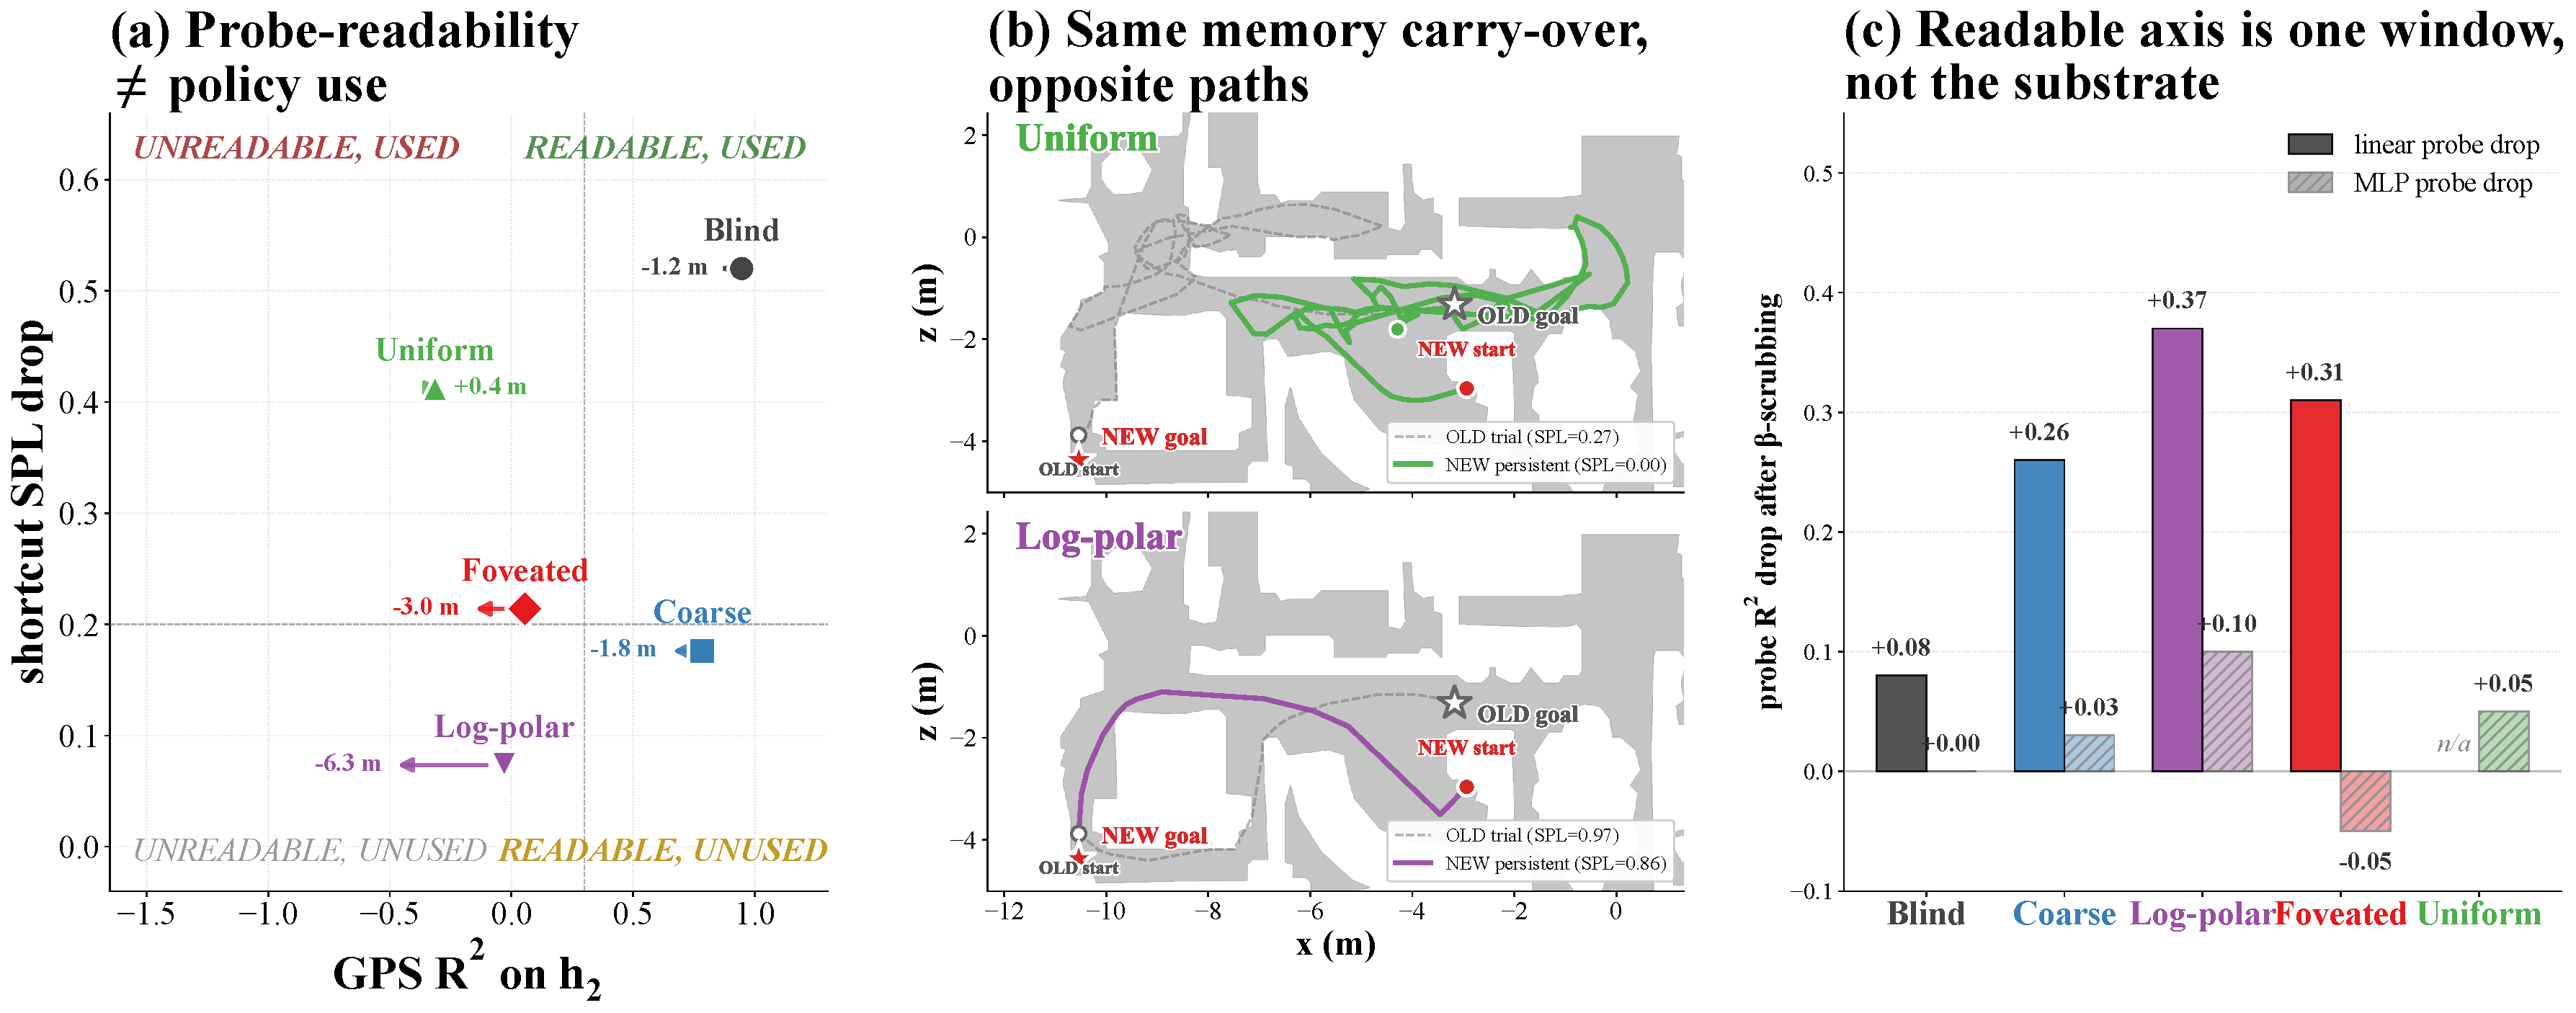
\includegraphics[width=\linewidth]{fig/fig5_consumption.pdf}
\caption{\textbf{Probe-readable position is not what drives behaviour.} \emph{(a)} Each condition's $(x{=}\text{GPS }R^2,\,y{=}\text{shortcut SPL drop})$ position locates it in the readability--reliance plane. The horizontal arrow encodes the per-condition median paired-episode pull margin $d(\text{end},\text{new}){-}d(\text{end},\text{old})$ on same-floor persistent-failure episodes: rightward indicates ``locks old'', leftward indicates ``tries new'', length is proportional to $|$median$|$. Only Uniform's arrow points right. \emph{(b)} \emph{Two trajectories diverge under identical setup}: Uniform fails to navigate to NEW-goal (its persistent memory pulls it toward OLD-goal area), Log-polar succeeds. Top-down trajectories on one scene's navmesh for the paired episode with the sharpest contrast in (a). Same scene, same paired (OLD, NEW) episode pair, same memory carry-over from OLD to NEW; only the visual encoder differs across the two panels. Each episode has its own independently-sampled start and goal (so OLD-start $\neq$ NEW-start, OLD-goal $\neq$ NEW-goal); the diagnostic question is where the NEW persistent trajectory ends relative to OLD-goal vs.\ NEW-goal. \emph{Top:} Uniform's NEW persistent path circles back near OLD-goal ($1.2$\,m from OLD-goal, $6.8$\,m from NEW-goal). \emph{Bottom:} Log-polar's path converges on NEW-goal ($8.0$\,m from OLD-goal, $0.0$\,m from NEW-goal). Dashed grey: OLD trial (faded, for context); solid colour: NEW persistent. \emph{(c)} Drop in probe $R^2$ after $\beta$-subspace scrubbing. We fit a Ridge $\beta$ that linearly predicts $(x,y)$ from $\mathbf{h}_2$, then project $\mathbf{h}_2$ orthogonally to $\beta$ at inference. Filled bars: linear probe drop (the ablation collapses the readable axis where it existed). Hatched bars: MLP probe drop (tiny across conditions, so non-linear decoders still recover position from non-$\beta$ directions). Uniform's linear bar is omitted because its original linear $R^2$ was already negative noise, so a post-scrubbing change there is uninterpretable.}
\label{fig:consumption}
\label{fig:consumption_summary}
\label{fig:shortcut_paired_traj}
\label{fig:scrubbing}
\end{figure}

A linear probe reveals what memory stores; it does not verify what the policy actually relies on. To test this, we need an intervention that asks the policy a question it can only answer with its memory: when memory is helpful, does taking it away hurt? Inspired by Tolman's same-scene cognitive-map test~\citep{tolman1948cognitive}, we run successive eval episodes within each scene under two memory regimes: in the \texttt{persistent} regime the LSTM hidden state carries over between episodes, and in the \texttt{reset} regime it is zeroed before each. Each episode is sampled independently (its own start, its own goal), so consecutive episodes within a scene differ in target. The SPL penalty of \texttt{persistent} relative to \texttt{reset} measures how much the policy leans on memory carry-over.

\noindent Two off-diagonal cases dissociate readability from reliance (Figure~\ref{fig:consumption}a): coarse carries a strong linear position code yet shows little reset penalty (``readable but unused''); uniform carries no linear code yet shows the largest reset penalty (``unused but readable via a substitute''). They raise distinct questions --- \emph{what is uniform reading instead of position?} and \emph{is the readable axis where the policy actually reads?} --- which two interventions answer.

\noindent\textbf{What is uniform reading?}\quad When a persistent agent fails the new task, it either drifts toward the old goal (``locks old'') or struggles around the new one (``tries new''). The signed margin $d(\text{end},\text{new}){-}d(\text{end},\text{old})$ (horizontal arrows in Figure~\ref{fig:consumption}a) separates the two regimes: only uniform points right (locks old; median $+0.43$\,m); blind, coarse, foveated, and log-polar all point left, increasingly so. Figure~\ref{fig:consumption}b shows the contrast on a single scene. What uniform reads looks more like \emph{which scene} than \emph{where in the scene}: a linear scene-id classifier on $\mathbf{h}_2$ separates scenes far better in sighted than in blind. \uncertain{The simplest reading is a scene-history anchor: ``head to where I was going last time I was in this scene''.}

\noindent\textbf{Is the readable axis the substrate?}\quad The coarse off-diagonal raises the converse worry: maybe the linear axis is \emph{epiphenomenal} --- correlated with position but not what the policy uses. We ablate it directly: fit a Ridge $\beta$ predicting $(x,y)$ from $\mathbf{h}_2$, project $\mathbf{h}_2$ orthogonally to $\beta$ at inference. The ablation collapses the linear probe but barely moves the MLP probe (Figure~\ref{fig:consumption}c; $\Delta R^2 \in [-0.05, +0.10]$): position is distributed redundantly across many directions, with the readable axis one window into a population code rather than its substrate --- the redundancy familiar from biological place-cell systems~\citep{stringer2019high}. Read this way, the dissociation in (a) is what we should expect: \emph{readable} and \emph{used} can come apart in either direction.

Two controls affect all conditions equally. Memory-init transplant (re-initialise from the previous-episode end-state rather than zero) drops SPL uniformly: persistent memory is an \emph{activity-slot} store bound to trajectory dynamics~\citep{dorrell2024taleoftwo}, not synaptic. GPS$+$compass ablation from step~0 collapses success to near-zero, confirming GPS as the upstream causal input. Full $4{\times}4$ catalog in Appendix~\ref{app:probing-details}.


\section{Discussion}
\label{sec:discussion}

\noindent\textbf{Three views of capacity allocation}\quad A reader could imagine three independent things happening across our five conditions: they differ in how much position lives in memory (magnitude, §\ref{sec:h1}), in the form that position takes (format, §\ref{sec:format-spatial}--§\ref{sec:tgm}), and in whether the policy actually uses it (consumption, §\ref{sec:dissociation}). We read the three as views of one allocation: the visual encoder and the integration of the position sensor compete for finite memory capacity, and visual bandwidth tilts the balance. Bottleneck conditions retain a linear position code in memory; rich-encoder conditions reallocate to the visual route; the policy reads from whichever route the memory makes available. Blind sits alone with a linearly-readable, format-isolated code and the largest behavioural reliance on its memory carry-over; uniform, foveated, and log-polar cluster as non-linear-only, format-shared codes; coarse falls off-diagonal (linearly-readable but format-shared), the configuration that triggers the dissociation in §\ref{sec:dissociation}. \uncertain{Coarse and uniform end up on opposite sides of the magnitude axis for different reasons: coarse's encoder cannot supply spatially-resolved features, so capacity defaults to the integration route; uniform's encoder supplies rich features that capture per-step position, so capacity is reallocated to the visual route, leaving integration unattended. The two are different regimes of one allocation, not the same mechanism.}

\noindent\textbf{Biological precedent}\quad The ``sensor format shapes spatial memory'' hypothesis has biological precedent~\citep{chen2016grid,geva2016remapping,fortin2008blind}: subterranean rodents that rely on integration rather than vision~\citep{kimchi2004molerat} parallel our blind agent; uniform's near-isotropic sampling parallels insect and zebrafish vision~\citep{geva2015spatial,toledo2020cognitive}; coarse's heavily-bottlenecked input parallels biological systems restricted to low-resolution environmental cues; and the cortical magnification structure of mammalian visual systems~\citep{strasburger2011peripheral,rosenholtz2016peripheral} parallels our log-polar control. Our results also align with the hidden-state inference framework of \citet{sanders2020remapping}: rich-encoder agents fail to generalise position codes across rooms (the LOSO result of §\ref{sec:format-spatial}), creating scene-specific hidden states that mimic biological global remapping, while bottleneck agents show no remapping. We do not claim direct biology--AI equivalence; we offer the parallel as a hypothesis the comparative-cognition literature can test by within-species manipulations of effective per-step visual variety (gaze restriction, dark-rearing, prosthetic compound vision).

\noindent\textbf{Implications and scope}\quad The principle is geometric: finite memory has fewer effective dimensions than its parameter count, and what those dimensions encode reflects a content-level competition between sensor sources. When the encoder pre-formats per-step features that already include position, memory reallocates capacity away from integration, eliminating the linearly-readable position code; under a bottleneck encoder, integration dominates and the linear code returns. This matches the Information Bottleneck invariance--disentanglement prediction~\citep{tishby2000ib,achille2018invariance}: bandwidth-restricted memory drives representations toward scene-invariant rather than scene-conditional encoding (Figure~\ref{fig:format_axis}b). The principle should also be architecture-level: any system where finite-capacity memory reads a pretrained encoder should show the same competition, regardless of whether ``memory'' is recurrent state or attention over history. In transformer-based navigators (e.g.\ \citealt{zeng2024poliformer}; cf.\ \citealt{whittington2022transformerhippocampus}), the principle predicts attention-readable position codes under bottleneck encoders and attention-internal, only non-linearly decodable codes under rich encoders, a direct falsification target. The same logic re-frames recent VLM spatial-reasoning failures~\citep{ramakrishnan2025space}: rich pretrained encoders may divert capacity away from the downstream substrate's spatial code rather than merely fail to teach it, so bandwidth-restricting perception may be \emph{cognition-enabling} rather than only compute-saving. As a partial architecture-independence test, we ported the design to a different environment, encoder family, and training regime: frozen DINOv2-Base~\citep{oquab2024dinov2} patch features at five resolutions feed a small recurrent memory trained on Memory Maze~\citep{pasukonis2023memorymaze} with next-feature prediction. The same dichotomy reproduces: the non-linear gap (MLP $R^2$ minus linear $R^2$) is monotone-decreasing with bandwidth (coarse $+0.62$ vs.\ uniform $+0.55$; Appendix~\ref{app:wmprobe}), in a setup that omits Habitat's GPS/compass channel and so isolates the format-shift dynamic from the bandwidth-allocation tradeoff.

\noindent\textbf{Limitations}\quad We evaluate a single training seed per condition (a convention from comparative-cognition modelling~\citep{wijmans2023emergence,banino2018grid,cueva2018grid,schaeffer2023grid}). Convergent multi-method evidence (geometrical, behavioural, and informational metrics ranking conditions identically, plus an independent blind replication; Appendix~\ref{app:repro}) argues against single-seed noise as the explanation, but multi-seed confidence intervals remain necessary future work. The pipeline (LSTM + DD-PPO + PointGoal + ResNet-18) matches prior cognitive-modelling work for direct comparability~\citep{wijmans2023emergence,banino2018grid,cueva2018grid}. Whether the magnitude and format patterns generalise to transformer-based navigators, alternative RL algorithms, or other tasks (e.g.\ ObjectGoal) is the cleanest falsification target. The Memory-Maze partial test (Appendix~\ref{app:wmprobe}; different encoder family, environment, and training regime) replicates the format-shift dichotomy, arguing against a pipeline-specific origin (LSTM gating, DD-PPO, or our particular sensor stack); and cross-condition memory transplants (§\ref{sec:causal-intervention}) demonstrate the ordering behaviourally, independent of any probe methodology.

\section{Conclusion}
\label{sec:conclusion}

We demonstrate that an agent’s cognitive map format is not a static architectural given, but an emergent property shaped by its visual sensor's bandwidth. Under a finite memory budget, rich pre-formatted visual features preempt temporal integration, driving memory into a scene-dependent format. Conversely, restricting sensory bandwidth frees capacity to construct globally linear, integration-derived spatial maps. For embodied AI, this yields a counterintuitive design principle: perceptual bottlenecks are not merely compute-saving compromises, but actively cognition-enabling constraints.
Methodologically, our results expose a critical dissociation in mechanistic interpretability: the linear decodability of a representation does not guarantee its use by the downstream policy, underscoring the necessity of causal, comparative-population interventions. Ultimately, our capacity-allocation principle bridges AI and neuroscience, suggesting that biological dichotomies (e.g., place vs. view cells) emerge from distinct sensory ecologies rather than divergent architectures. This opens a new pathway to scale spatial reasoning in foundation models not just by adding data, but by strategically constraining perception.
% We propose that visual sensor structure fundamentally shapes the content of spatial memory rather than simply modulating computational load. Under a finite memory budget, the bandwidth of the encoder dictates the balance between pre-formatted visual features and recurrently constructed states. This coupled dynamic implies that bandwidth-restricting perception can be cognition-enabling rather than merely compute-saving. For instance, foveation frees memory capacity to construct the integration-derived spatial representations that high-capacity sensors preempt. Consequently, the long-standing contrast between place cells and view cells across species may emerge from a shared allocation principle operating under different sensor ecologies, rather than species-specific architectural differences.

% These results also offer a critical lesson for mechanistic interpretability: a linear probe might be able to identify a readable feature, but does not guarantee that the downstream task consumes it. Because probes merely capture correlational structure, true mechanistic claims rely on causal interventions. We show that \emph{comparative-population studies} (varying exactly one sensory constraint across matched agents) dramatically sharpen these tests. By observing how the same ablation triggers different behavioral signatures across conditions, we can systematically map how hardware bounds rewrite an agent's cognitive strategy. We see this as a step toward a comparative cognitive neuroscience of artificial agents, where the same population-geometry, intrinsic-timescale, and transplant-cost tools used to map biological cortex apply with the comparative variable held truly fixed in a way biology cannot easily realise.

\newpage
\bibliographystyle{plainnat}
\bibliography{literature}

\newpage
\input{checklist}

\newpage
\appendix

\section{Reproducibility: Hyperparameters and Implementation Notes}
\label{app:repro}

\noindent\textbf{Training hyperparameters (DD-PPO, all five conditions identical)}\quad
8-GPU \texttt{torchrun} on a single 8$\times$A100 node; \texttt{num\_steps=256}, learning rate \texttt{lr=2.5e-4} with \texttt{lr\_decay=False}; \texttt{num\_environments=16/worker}; total budget 250M frames per condition. All other hyperparameters follow the Habitat-baselines DD-PPO defaults from \citet{wijmans2020ddppo}.

\noindent\textbf{Architectural details (sensor encoding)}\quad
Each non-visual sensor (goal-in-start-frame, GPS, compass, close-to-goal scalar) is projected to 32-d via a per-sensor linear layer; the previous-action embedding is also 32-d (\texttt{nn.Embedding} with action-space cardinality + 1 for the no-prev-action token). The four sensor projections are concatenated with the previous-action embedding and the (flattened) visual encoder output to form the LSTM Layer-0 input vector. This matches the \citet{wijmans2020ddppo} Wijmans-default sensor stack.

\noindent\textbf{Implementation notes (foveated condition)}\quad
The foveated condition disables the running-mean-and-variance input normaliser (a per-channel running normalisation layer applied to the visual stream before the ResNet-18 backbone) to avoid an in-place autograd conflict between the running-buffer update and the foveation-blur backward pass. Behavioural success and SPL are unaffected by this choice; an ablation that re-enables the normaliser (with the autograd conflict patched) is available for future work that wants to revisit it.

\noindent\textbf{Implementation notes (numerical stability)}\quad
Two safeguards protect against rare numerical instabilities arising from off-navmesh episodes: (i)~a pre-update gradient sanitisation pass replaces NaN/Inf gradients with zero before each PPO step; (ii)~a forward-looking geodesic-distance clamp prevents reward NaNs when the agent steps off the navmesh. Both are no-ops on healthy trajectories and apply identically to all five conditions.

\noindent\textbf{Log-polar foveation transform}\quad
The log-polar control (Appendix~\ref{app:scaling}) applies a differentiable log-polar resampling step before the ResNet-18 backbone: the $128{\times}128$ avg-pooled image is mapped onto a $64{\times}64$ grid with $n_\rho{=}64$ log-spaced radial samples and $n_\theta{=}64$ angular samples, mimicking the cortical magnification of mammalian primary visual cortex. Visual front-end only; LSTM, sensors, and training pipeline are identical to the foveated condition.


\section{Probing Protocol Details}
\label{app:probing-details}

\noindent\textbf{Sampling protocol}\quad An earlier draft used stochastic (policy-distribution) action selection at probe time. Conditions with higher action-entropy under their trained stochastic policies sampled the STOP action early with $\sim 0.25$ per-step probability, producing $\sim 4$-step rollouts and target variance two orders of magnitude below the episodic range. The resulting probe $R^2$ values were trivially high across all conditions (any predictor fits a near-constant target). This confounded cross-condition comparisons; we switched to the deterministic (argmax) protocol used here and elsewhere in our pipeline. All paper results use the deterministic protocol.

\noindent\textbf{Length-matching ablation}\quad Under deterministic rollouts, episode lengths span $\sim$100--400 mean steps depending on condition. We use 5-fold episode-level CV to keep splits balanced per scene rather than length-matching across conditions. A controlled length-matching ablation (truncate every condition to a common length) is left for follow-up; we expect the magnitude ordering to be preserved because bottleneck conditions decode at high $R^2$ even at the smallest sub-sample, but have not verified.

\noindent\textbf{Cross-heading probe}\quad The proposal included a cross-heading generalisation probe (train on heading $A$, test on opposite heading). Our implementation returned ``insufficient samples'' sentinels at our probe sizes; not in our results.

\noindent\textbf{LSTM Layer~0 sensor branch}\quad The non-visual sensor stack (goal-in-start-frame, GPS, compass, close-to-goal scalar, prev-action) projects each sensor to 32-d, concatenates them with the visual encoder's flattened output, and feeds the result as the LSTM's Layer~0 input. The GPS embedding therefore enters the LSTM via this concatenation; this explains why Figure~\ref{fig:magnitude}c shows linearly-decodable GPS at Layer~0 even for conditions whose visual encoder discards GPS entirely. Per-layer probes show the same pattern at every hidden-state layer: Layer~0 carries GPS for every condition; Layer~1 dips for everyone; Layer~2 separates blind/coarse from foveated/uniform. Cell states $\mathbf{c}_\ell$ do not carry the GPS code as cleanly as hidden states ($\mathbf{c}_1$ at chance/negative for every condition; $\mathbf{c}_2$ positive only for blind, $R^2 \approx +0.57$). The headline ``top-layer linearly-decodable GPS'' claim is therefore specifically about $\mathbf{h}_2$, not the cell pathway.

\noindent\textbf{Non-linear (MLP) probe details}\quad For each condition we fit a 2-layer MLP (hidden $256{-}128$, ReLU, $L_2$ weight decay $10^{-4}$, sklearn \texttt{MLPRegressor} with early-stopping) on the same top-layer hidden states and GPS labels as the linear Ridge probe, with the same 5-fold episode-level CV. The full probe-depth sweep (linear $\to$ MLP-1 $\to$ MLP-2 $\to$ MLP-4) shown in Figure~\ref{fig:format_axis}a establishes a depth-graded recovery: bottleneck conditions plateau near $R^2 \approx 0.95$ from depth-0 (linear suffices), while rich-encoder conditions ramp up sharply with probe depth. Top-layer MLP-2 recovery (Ridge linear $\to$ MLP-2): blind $0.92 \to 0.98$, coarse $0.51 \to 0.75$, foveated $0.06 \to 0.79$, log-polar $-0.07 \to 0.63$, uniform $-2.28 \to 0.35$. The MLP probe alone cannot disentangle ``non-linear position code'' from ``MLP regressing through position-correlated features (wall distance, scene identifiers, episode-phase markers)''; the log-polar foveation control (Appendix~\ref{app:scaling}) targets that question at one intermediate point.

\section{Alternative-Account Explainations}
\label{app:alt-accounts}

\emph{Task-competence differences.} All sighted conditions solve PointGoal at $93$--$99\%$ success and blind at $76\%$ (Table~\ref{tab:summary}); all five conditions converge behaviourally well before the probing window, so the encoded-content gap cannot be attributed to navigation skill or differential under-training.

\emph{Probe-capacity / probe-fitting artefacts.} A direct test: distance-to-goal (DtG) decodes robustly across all five conditions ($R^2 \geq 0.88$; Figure~\ref{fig:supp_goal_vec}) while the goal-direction component is at chance everywhere (PointGoal provides the goal vector as a per-step input, so the policy has no incentive to re-encode it). The linear probe is therefore capable of fitting position-correlated structure when it exists; the chance-level rich-encoder GPS $R^2$ is a hidden-state property, not a probe artefact. The real-vs-permuted-label gap (Hewitt--Liang selectivity) likewise tracks GPS $R^2$.

\emph{Sample-size / trajectory-distribution artefacts.} CV $\sigma$ spans come from the same 500-episode pool with $\sim 100$--$400$-step rollouts under identical deterministic evaluation; the protocol confound that haunted an earlier draft is documented and retired in Appendix~\ref{app:probing-details}.

\emph{Linear-probe artefacts.} Three complementary checks. \emph{(a)~Behavioural:} the memory-transplant intervention goes outside the probe framework and reproduces the bottleneck-vs-rich-encoder ordering; the $5\times 5$ matrix's asymmetry adds structure no linear-similarity measure can read. \emph{(b)~Non-linear (MLP) probe:} a 2-layer MLP recovers $R^2 \in [0.35, 0.79]$ from rich-encoder top-layer states (Appendix~\ref{app:probing-details}). \emph{(c)~Non-linear similarity.} Beyond linear similarity (off-diagonal CKA~\citep{kornblith2019cka} $< 10^{-4}$), a non-linear t-SNE embedding also separates the five conditions with 1-NN purity $1.000$ vs.\ chance $0.20$ --- the format divergence is not an artefact of linear-similarity measures. H1 is therefore specifically about \emph{linear} top-layer readability --- what the linear DD-PPO action head can consume --- not GPS absence.


\section{Magnitude: Corroborating Diagnostics}
\label{app:magnitude-detail}
\label{app:mine}

To anchor the information-allocation finding in §\ref{sec:h1} on a nat-scale rather than the bounded, model-dependent $R^2$ scale of probes, we estimate $I(\mathbf{h}_2; \text{pos})$ per condition using the Mutual Information Neural Estimator~\citep{belghazi2018mine}. We fit a 3-layer MLP critic ($256$ hidden, ELU, batch $512$, lr $10^{-4}$, $4{,}000$ steps) on joint $(\mathbf{h}_2, \text{pos})$ samples vs.\ within-batch shuffled marginals, with the bias-corrected gradient (eq.~12 of \citealt{belghazi2018mine}). Final $I(\mathbf{h}_2; \text{pos})$ in bits (mean $\pm$ std across 3 seeds): blind $6.01 \pm 0.06$, coarse $4.55 \pm 0.03$, log-polar $4.66 \pm 0.04$, foveated $4.30 \pm 0.04$, uniform $4.47 \pm 0.06$. Total mutual information decreases with encoder bandwidth, but the decrease is gentle ($\approx 1.3\times$ blind/uniform) compared to the linear-probe $R^2$ collapse (effectively factor-of-zero for uniform). The within-sighted ordering is reproducible across seeds (per-condition std $\leq 0.06$ bits, much smaller than the within-sighted gap $\approx 0.36$); the dominant signal is the bottleneck-vs-rich-encoder gap (blind $6.01$ vs sighted mean $4.49$). Interpretation: rich-encoder conditions retain substantial position information in $\mathbf{h}_2$, but it is encoded non-linearly and partly offloaded to the encoder route, paralleling the LOSO scene-invariance result (Figure~\ref{fig:format_axis}b).


\section{Spatial Format: Corroborating Diagnostics}
\label{app:format-spatial-detail}

This appendix collects spatial-format diagnostics in four consolidated figures: convergent format-divergence metrics (Figure~\ref{fig:format_divergence}); capacity-allocation geometry within $\mathbf{h}_2$ (Figure~\ref{fig:capacity_geometry}); eigenspectrum (Figure~\ref{fig:eigen_scrub}); and the goal-vector probe (Figure~\ref{fig:supp_goal_vec}). The $\beta$-subspace scrubbing intervention is reported in main-text Figure~\ref{fig:consumption}c. All panels report the full 5-condition set.

\begin{figure}[!t]
\centering
\begin{minipage}[c]{0.50\linewidth}\centering
  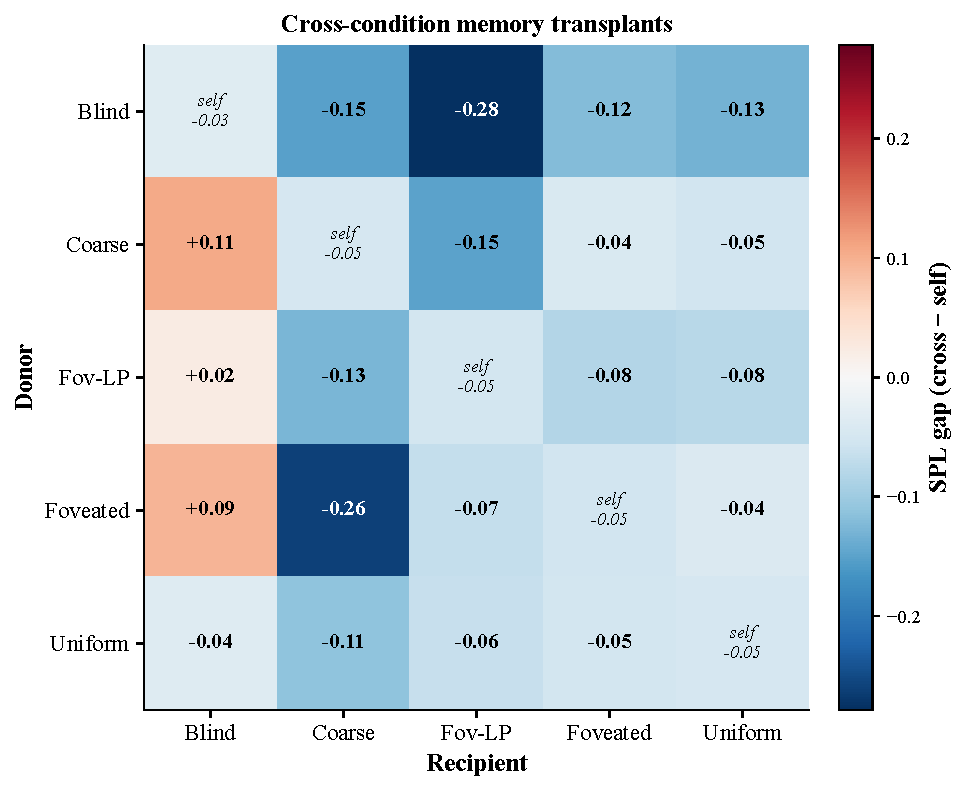
\includegraphics[width=\linewidth]{fig/figa7a_transplant_5x5.pdf}\\[-2pt]
  {\footnotesize\textbf{(a) $5{\times}5$ memory-transplant matrix}}
\end{minipage}\hfill
\begin{minipage}[c]{0.48\linewidth}\centering
  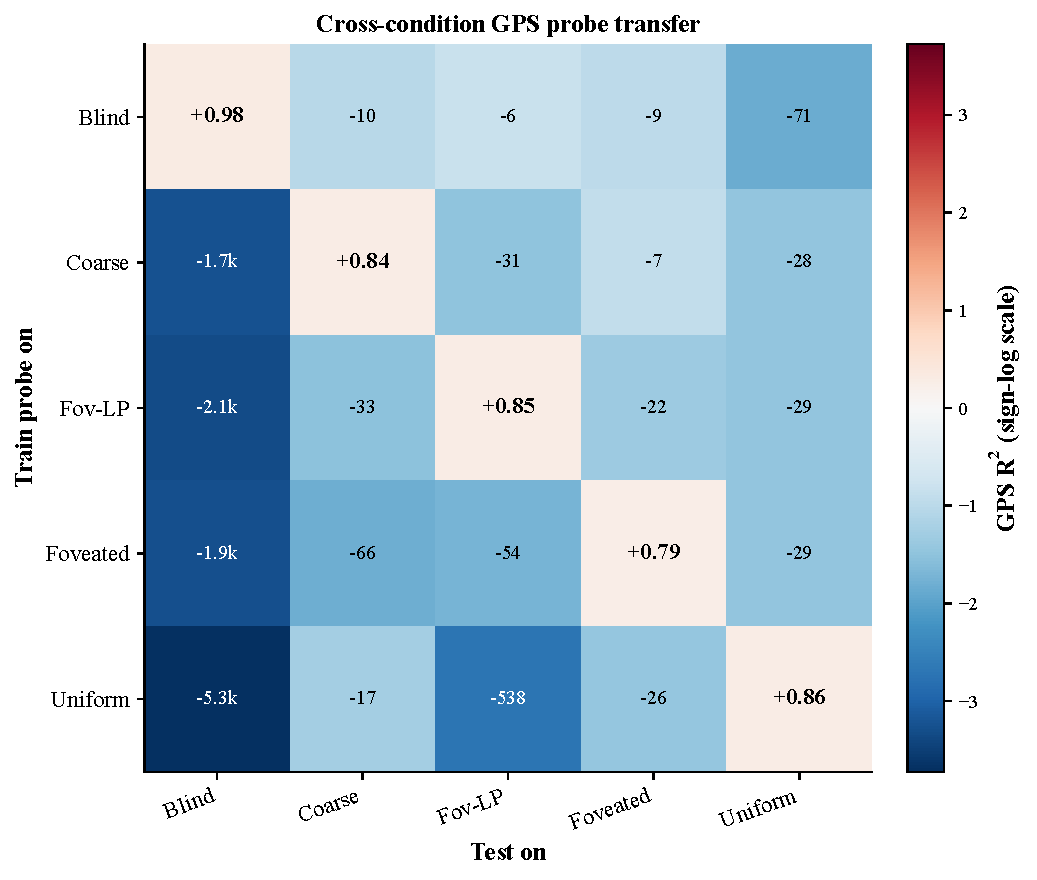
\includegraphics[width=\linewidth]{fig/figa7b_h2_probe_transfer.pdf}\\[-2pt]
  {\footnotesize\textbf{(b) Cross-condition probe transfer}}
\end{minipage}
\caption{\textbf{Two corroborating views of format divergence.} \textbf{(a)} Full $5{\times}5$ memory-transplant matrix at midpoint $t{=}30$. Per-recipient column means enter main Figure~\ref{fig:format_axis}b as the transplant-cost axis; the matrix exposes the underlying direction-asymmetry. \textbf{(b)} Cross-condition probe-transfer matrix: train a Ridge GPS probe on the row condition, test on the column. Off-diagonal $R^2$ is strongly negative (clipped to $[-1, 1]$ for display; raw values $-3.5{\times}10^2$ to $-3.5{\times}10^4$): position-axes are jointly incompatible at the readout level even though every condition visits the same scenes and solves the same task.}
\label{fig:format_divergence}
\label{fig:format_appendix}
\end{figure}

\begin{figure}[!t]
\centering
\begin{minipage}[t]{0.32\linewidth}\centering
  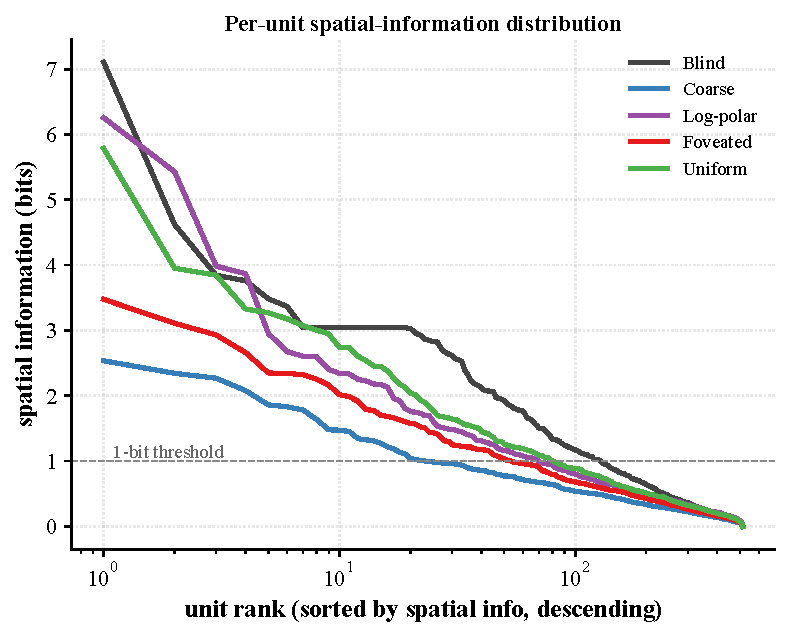
\includegraphics[width=\linewidth]{fig/figa9a_per_unit_info.pdf}\\[-2pt]
  {\footnotesize\textbf{(a) Per-unit spatial info}}
\end{minipage}\hfill
\begin{minipage}[t]{0.32\linewidth}\centering
  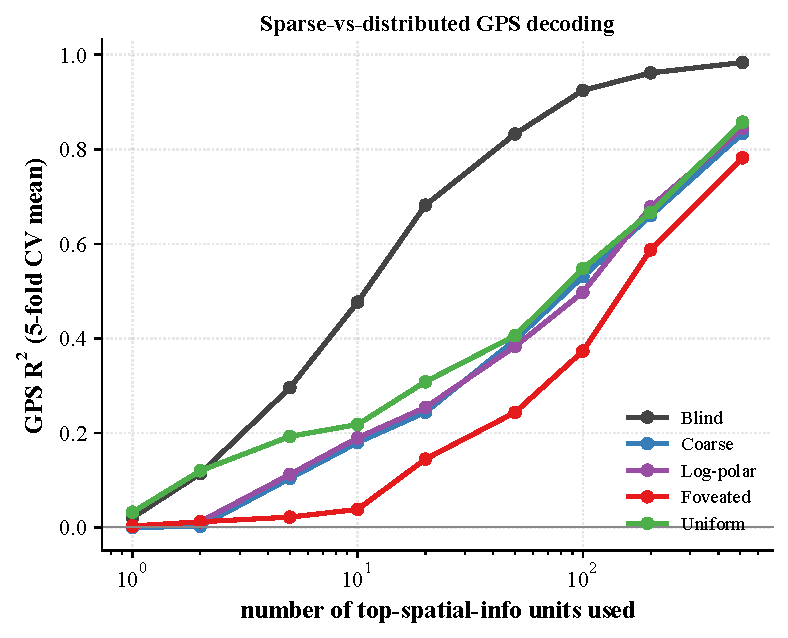
\includegraphics[width=\linewidth]{fig/figa9b_sparse_decoding.pdf}\\[-2pt]
  {\footnotesize\textbf{(b) Sparse-vs-distributed GPS decoding}}
\end{minipage}\hfill
\begin{minipage}[t]{0.32\linewidth}\centering
  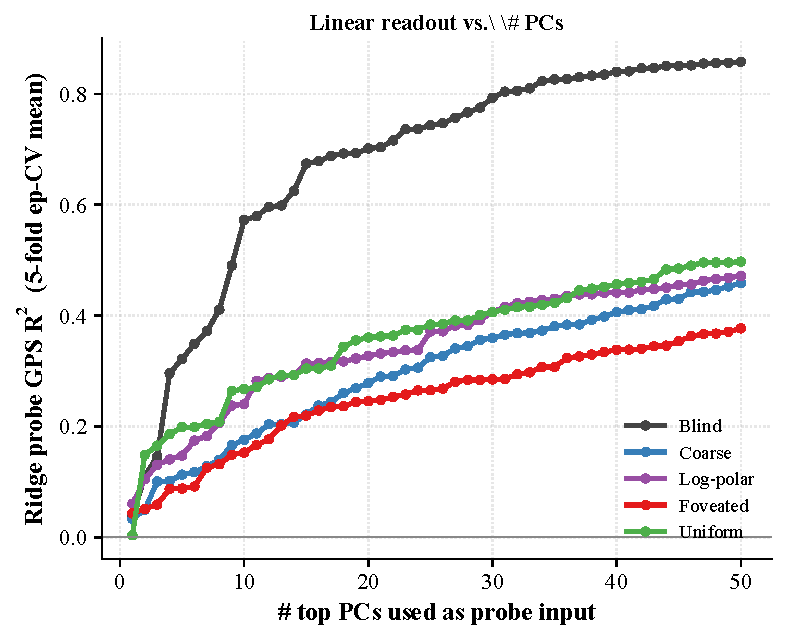
\includegraphics[width=\linewidth]{fig/figa13_pc_cumulative.pdf}\\[-2pt]
  {\footnotesize\textbf{(c) Linear readout vs.\ \# PCs}}
\end{minipage}
\caption{\textbf{Capacity-allocation geometry within $\mathbf{h}_2$.} Three views of the same population structure: bottleneck conditions concentrate the position code on a few axes, rich-encoder conditions distribute it across many. \textbf{(a)} Per-unit spatial-information distribution (units sorted descending; log $x$). Rich-encoder conditions hold a few units with marginally higher peak spatial info ($\approx 2$ bits) than bottleneck conditions. \textbf{(b)} GPS decodability from the top-$k$ spatial-info units: blind reaches $R^2 \approx 1.0$ at small $k$; rich-encoder networks fail at every $k$. Higher per-unit spatial information $\neq$ population position readout: peaked rich-encoder units encode features correlated with position (visual landmarks, trajectory phase), not position itself. \textbf{(c)} Ridge-probe GPS $R^2$ versus the number of top PCs of $\mathbf{h}_2$ used as input: blind plateaus by $\leq 10$ PCs (axis aligned with low-variance directions); rich-encoder $R^2$ barely climbs across $50$ PCs. The participation ratio $(\Sigma\lambda)^2/\Sigma\lambda^2$ varies across sighted conditions ($1.7$--$9.1$) without tracking encoder bandwidth monotonically.}
\label{fig:capacity_geometry}
\label{fig:supp_pop_coding}
\end{figure}

\begin{figure}[!t]
\centering
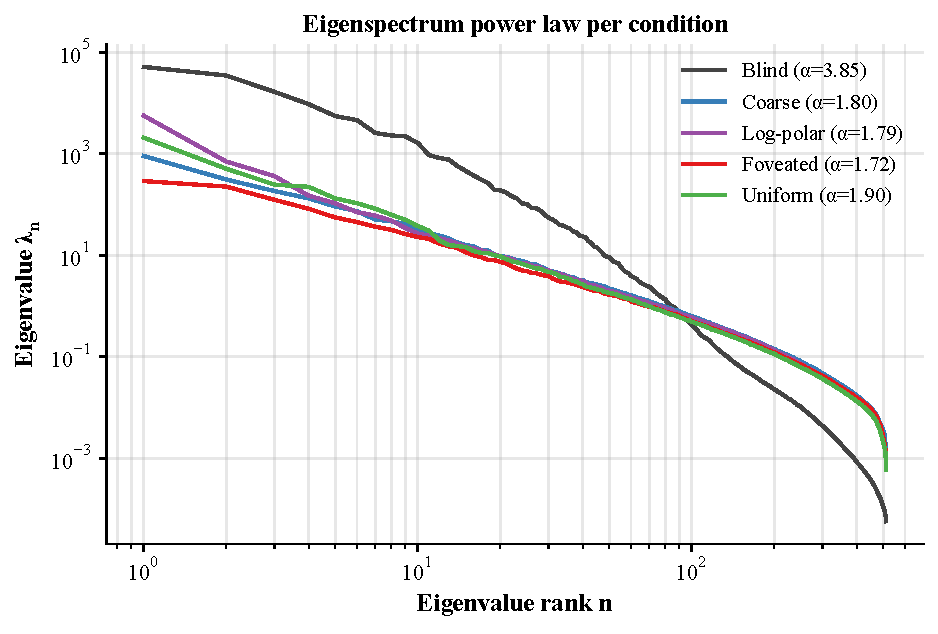
\includegraphics[width=0.55\linewidth]{fig/figa15_eigenspectrum.pdf}
\caption{\textbf{Eigenspectrum of $\mathbf{h}_2$: geometric reading of capacity allocation.} Log--log eigenvalue $\lambda_n$ vs.\ PC index $n$, with reference exponents $\alpha{=}1$ (Stringer V1) and $\alpha{=}1+2/3$ (smoothness/efficiency border at $d_{\rm task}{=}3$); per-condition $\alpha$ fitted on log-$\lambda_n$ vs.\ log-$n$, PCs $5$--$200$. Blind sits well above the critical exponent ($\alpha \approx 3.85$; top-10 PCs hold $95\%$ of variance), a few-direction concentrated regime; the four sighted conditions cluster around $\alpha \approx 1.7$--$1.9$, spreading variance across more directions. The split mirrors the magnitude split (§\ref{sec:h1}) at the geometric level: blind's reliance on the integration route yields a low-dimensional spectrum; sighted conditions spread variance to support encoder-route information.}
\label{fig:eigen_scrub}
\label{fig:eigenspectrum}
\end{figure}


\begin{figure}[!t]
\centering
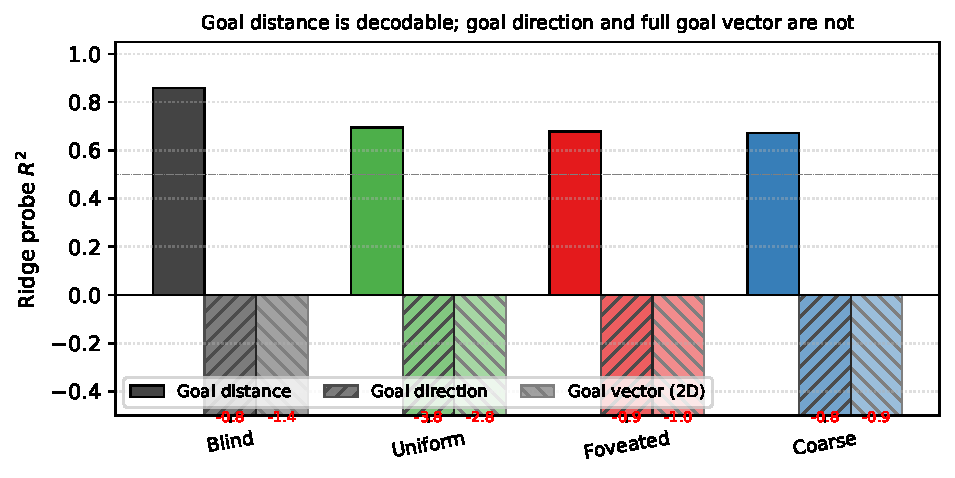
\includegraphics[width=0.65\linewidth]{fig/figa10_goal_vector.pdf}
\caption{\textbf{Goal-vector probe $R^2$ across all five conditions.} Goal distance (DtG) decodes strongly everywhere ($R^2 \in [0.89, 0.96]$; 5-fold episode-level CV); goal direction and the full ego-frame goal vector are at chance or negative for every condition. PointGoal provides the goal vector as a per-step input, so the policy has no incentive to re-encode it. The probe is therefore capable of reading position-correlated structure when it exists; the chance-level rich-encoder GPS $R^2$ is a hidden-state property, not a probe artefact.}
\label{fig:supp_goal_vec}
\end{figure}

\section{Temporal Format: Corroborating Diagnostics}
\label{app:format-temporal-detail}

This appendix collects two further diagnostics referenced from §\ref{sec:tgm}: a topological-distinguishability test via persistent homology (Section~\ref{app:topology}) and a predictive-horizon test grounded in successor-representation theory (Section~\ref{app:predictive_horizon}). One note on the main-text intrinsic-timescale view (Figure~\ref{fig:temporal_format}b): within sighted, the four conditions cluster near-identically at the per-unit autocorrelation level ($\tau \approx 7$--$8$ vs.\ blind's $\tau \approx 12$); the within-sighted bandwidth-inverse stiffness signal lives in the decoder-decay view (Figure~\ref{fig:temporal_format}c) rather than in per-unit timescale.

\subsection{Topological Distinguishability via Persistent Homology}
\label{app:topology}

A parameter-free pipeline used for toroidal grid-cell structure in mouse cortex~\citep{gardner2022toroidal} confirms that conditions are topologically distinguishable. Persistent $H_1$ loop counts order monotonically with encoder bandwidth: blind $219$, coarse $203$, log-polar $183$, foveated $152$, uniform $133$. Cross-condition Wasserstein-2 distance between $H_1$ persistence diagrams ($\sim 15$--$20$\,dgm$_1$) is roughly $2{\times}$ the within-condition seed noise ($\sim 8$--$11$\,dgm$_1$) for every condition, so the $\mathbf{h}_t$ manifolds are topologically distinguishable. We treat this as suggestive corroboration rather than independent mechanistic evidence. \uncertain{Our pre-registered prediction was the opposite direction (we expected uniform highest, blind lowest); we report what we found.}

\subsection{Predictive Horizon: Does $\mathbf{h}_t$ Encode Future Positions?}
\label{app:predictive_horizon}

Successor-representation theory~\citep{stachenfeld2017predictive,whittington2020tem} predicts that hippocampal place cells encode not just current position but a discounted future-occupancy code: place-cell firing at $s_t$ corresponds to expected visits to nearby states $s_{t+k}$. We test the analog claim for our recurrent state: does a linear probe from $\mathbf{h}_t$ recover \emph{future} positions $(x, y)_{t+k}$ for $k \in \{0, 1, 5, 10, 20, 50\}$?

\begin{center}
\begin{tabular}{l|cccccc}
\toprule
 & $k=0$ & $k=1$ & $k=5$ & $k=10$ & $k=20$ & $k=50$ \\
\midrule
\multicolumn{7}{l}{\emph{Linear (Ridge $\alpha = 10$) $R^2$, all-episode pooling, episode-level 5-fold CV}} \\
Blind             & $+0.94$ & $+0.94$ & $+0.94$ & $+0.92$ & $+0.90$ & $+0.79$ \\
Coarse            & $+0.57$ & $+0.57$ & $+0.57$ & $+0.56$ & $+0.50$ & $+0.37$ \\
Foveated          & $+0.06$ & $+0.06$ & $+0.08$ & $+0.13$ & $+0.19$ & $+0.06$ \\
Log-polar & $+0.17$ & $+0.18$ & $+0.17$ & $+0.11$ & $-0.14$ & $-0.50$ \\
Uniform           & $-4.31$ & $-4.32$ & $-4.32$ & $-4.26$ & $-4.39$ & $-10.14$ \\
\bottomrule
\end{tabular}
\end{center}

Blind exhibits a long predictive horizon: linear $R^2$ from $\mathbf{h}_t$ to $(x, y)_{t+k}$ remains $\geq 0.90$ from $k=0$ to $k=20$ (only $0.04$-point drop) and $0.79$ at $k=50$ --- the same linear projection that decodes current position at $R^2 = 0.94$ decodes positions $20$ steps in the future at $R^2 = 0.90$, a strong form of the predictive-map signature predicted by SR theory. Coarse follows at lower magnitude ($R^2 \in [0.50, 0.57]$ across $k=0$--$20$, $0.37$ at $k=50$). Rich-encoder conditions have no clear predictive horizon: foveated stays in $[0.06, 0.19]$ across all $k$ with no monotonic decay; log-polar starts at $+0.17$ and turns negative by $k=20$; uniform is already strongly negative at $k=0$ and grows more negative. Rich-encoder $\mathbf{h}_t$ encodes neither current nor future position linearly --- the LOSO scene-invariance reading of §\ref{sec:format-spatial} extended in time. The asymmetry: bottleneck conditions encode $\mathbf{h}_t$ as a smoothly-varying integrated GPS code that linearly predicts upcoming positions; rich-encoder conditions encode $\mathbf{h}_t$ reactively to the current visual scene without temporal extrapolation.


\section{Consumption: Corroborating Diagnostics}
\label{app:consumption-detail}
\label{app:causal-detail}

The main-text §\ref{sec:dissociation} reports the persistent-memory failure-mode test as the condition-discriminating intervention; this appendix presents two boundary-check interventions that characterise the consumption mechanism without separating conditions (Section~\ref{app:boundary-checks}), the full $5{\times}4$ failure-mode catalog spanning the per-condition margin distribution (Figure~\ref{fig:shortcut_catalog}), and a memory-transplant midpoint sweep that defends the $t{=}30$ choice in the main-text $5{\times}5$ transplant matrix (Figure~\ref{fig:transplant_sweep_supp}).

\subsection{Boundary Checks: Memory-Init Transplant and GPS-sensor Ablation}
\label{app:boundary-checks}

\emph{Memory-init transplant} (re-initialise memory from the previous-episode end-state instead of from zero) drops SPL by a comparable amount across all five conditions ($\Delta\text{SPL} \in [-0.10, -0.14]$). The cross-condition uniformity is itself the finding: every policy at $t{=}0$ expects a zero memory state, so memory in this architecture is an \emph{activity-slot} store~\citep{dorrell2024taleoftwo} bound to the trajectory dynamics, not a synaptic store. \emph{GPS$+$compass ablation} from step~0 collapses success from baseline ($0.81$--$0.98$) to near zero ($0.02$--$0.06$) across all five conditions ($\Delta \in [-0.75, -0.97]$): the position sensor is the upstream causal source whose integration memory encodes. The absolute drops cluster tightly across the four sighted conditions and do not cleanly separate them, consistent with the upstream sensor being a shared causal bottleneck rather than a discriminator.

\subsection{Persistent-Memory Failure-Mode Catalog}
\label{app:shortcut-catalog}

The main-text Figure~\ref{fig:shortcut_paired_traj} shows one canonical paired-episode case per condition; the full $5{\times}4$ catalog below shows four cases per condition (now including log-polar) spanning the per-condition margin range. Selection criterion: reset SPL $> 0.5$, persistent SPL $< 0.2$, persistent steps $\geq 30$, $|\Delta y_\text{goal}| < 0.5$\,m (same-floor old vs.\ new goal). Panels within each row are ordered by margin (left = most-negative = closer to new goal; right = most-positive = closer to old goal).

\begin{figure}[!t]
\centering
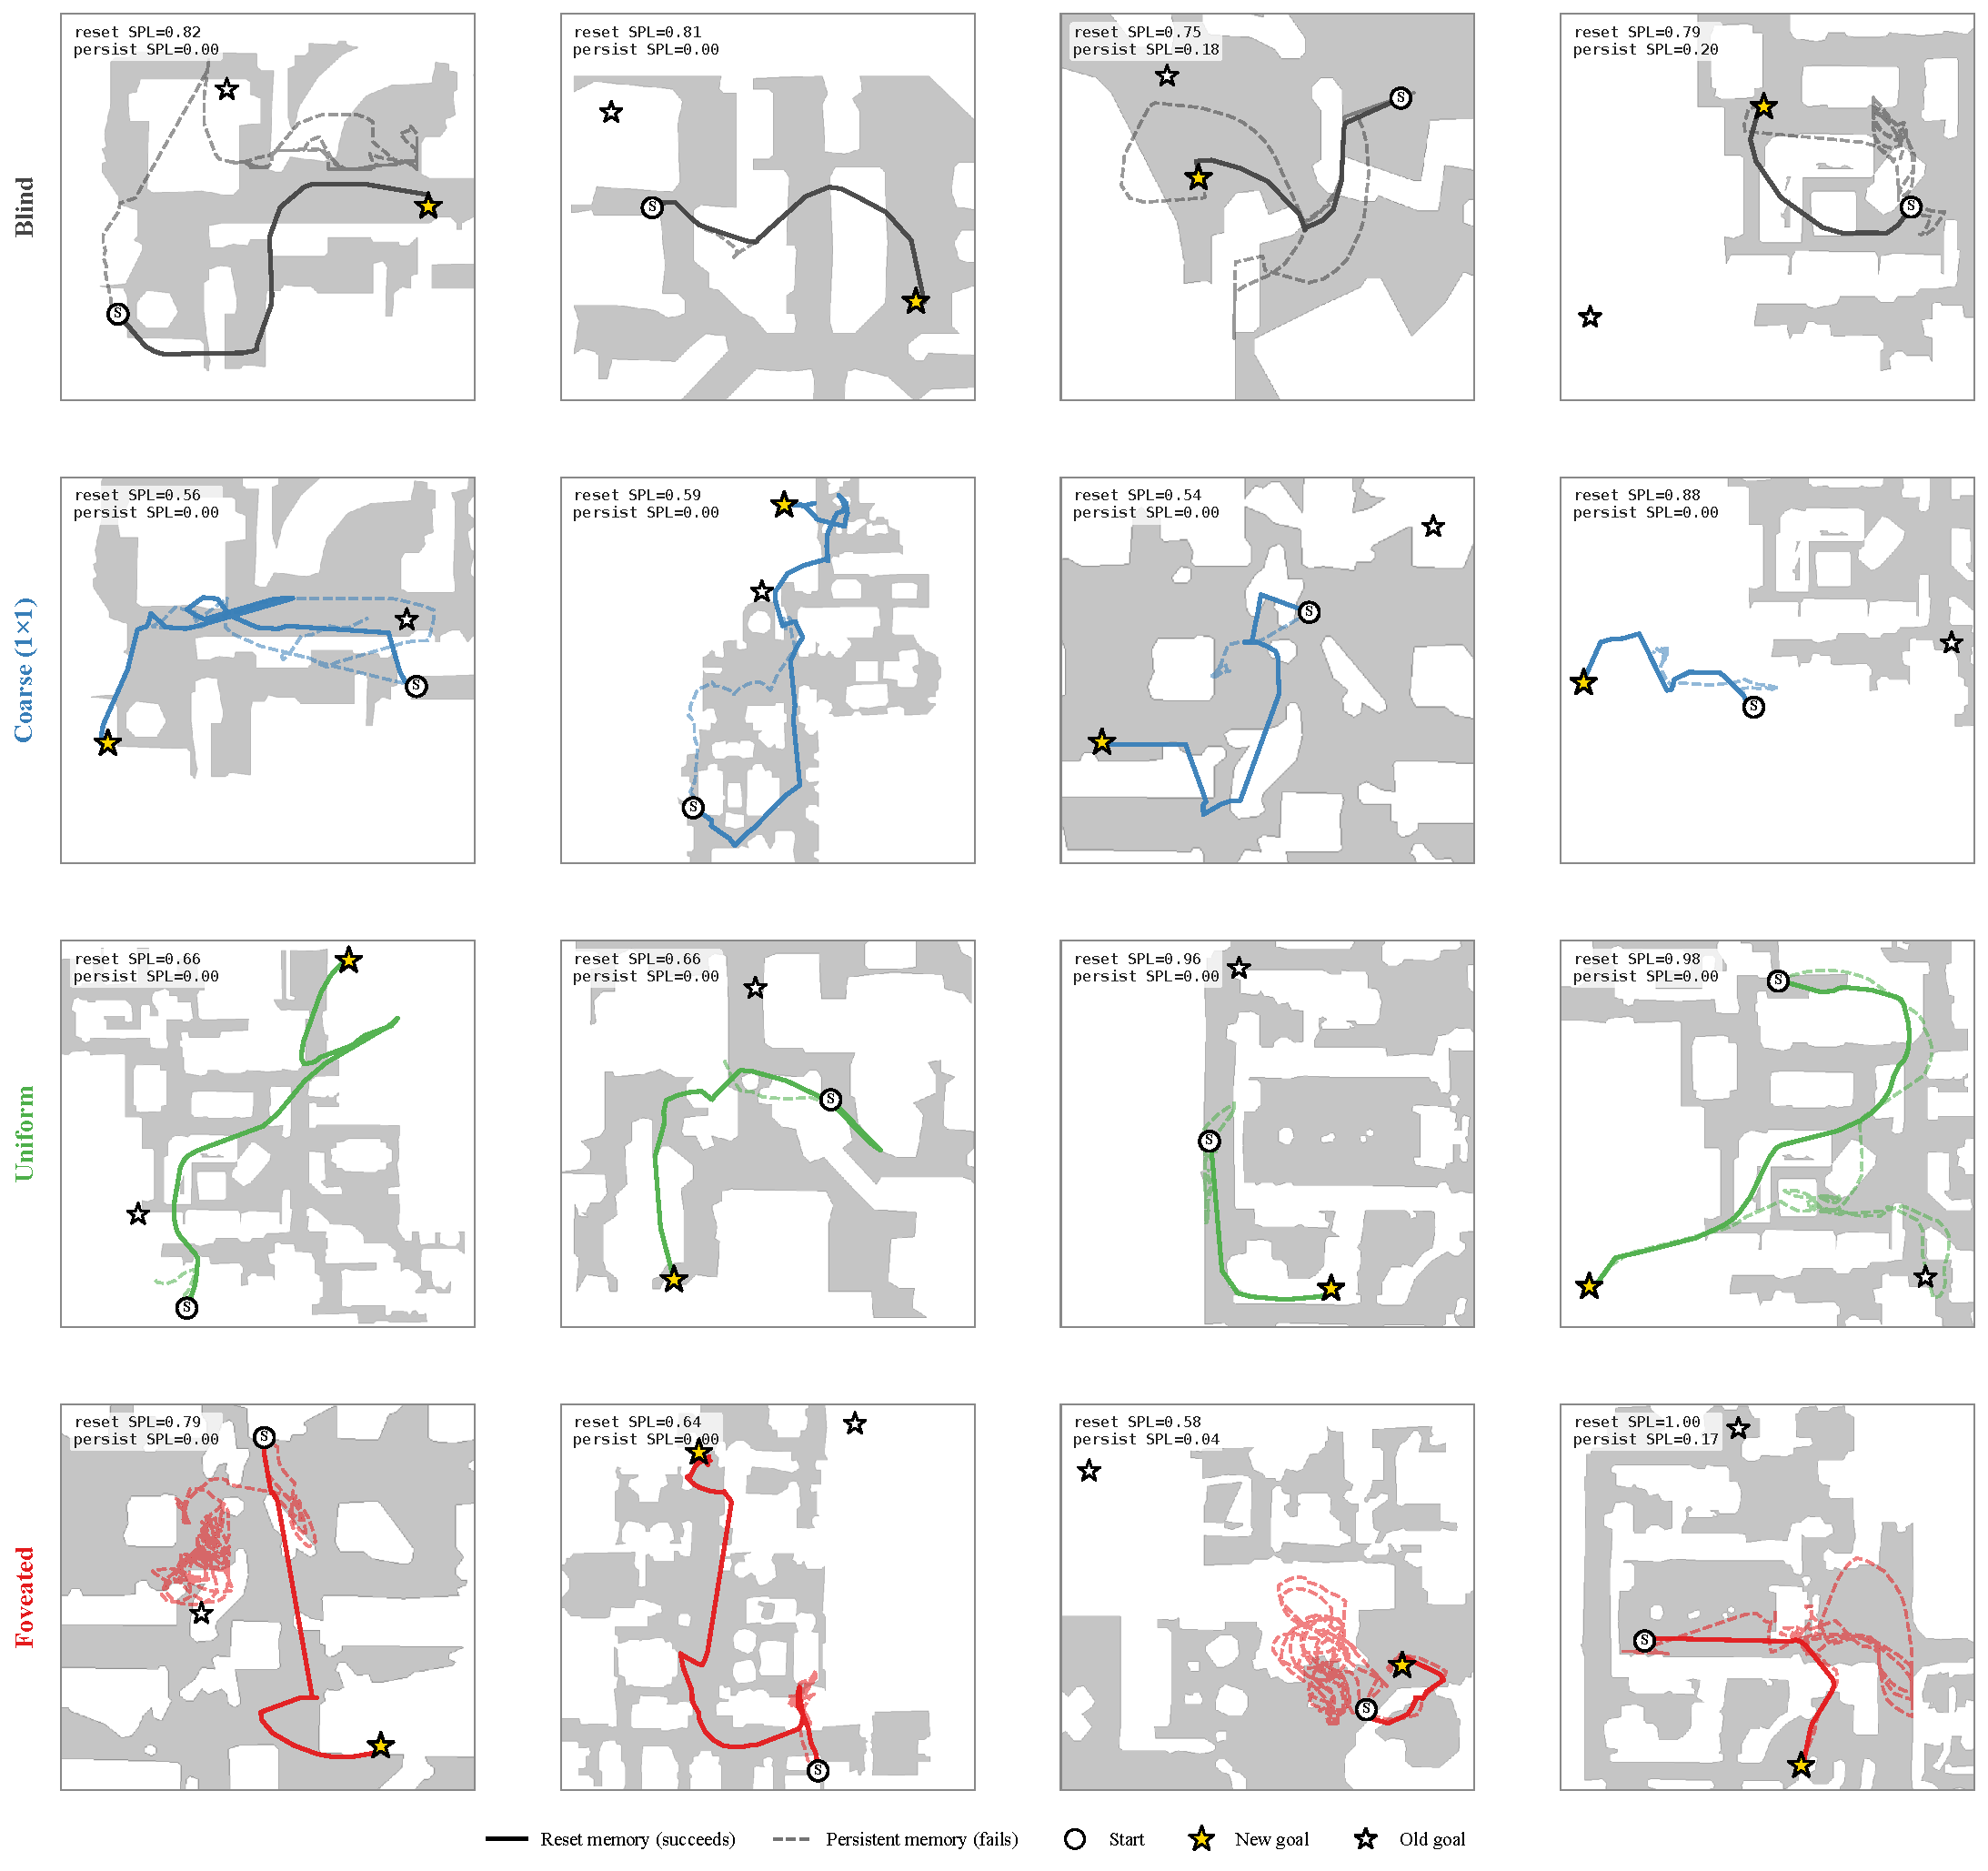
\includegraphics[width=\linewidth]{fig/figa17_shortcut_catalog.pdf}
\caption{\textbf{Persistent-memory failure-mode catalog: 4 cases per condition spanning the per-condition margin range.} Reset trajectory (solid, condition colour) reaches the new goal; persistent trajectory (dashed bold) shows where the persistent-memory agent ends up. Blind and Coarse cluster at ``tries-new''; Log-polar's persistent agent rarely fails outright, so all four selected cases skew tries-new; Uniform clusters at ``locks onto old''; Foveated is mixed.}
\label{fig:shortcut_catalog}
\end{figure}


\subsection{Memory-Transplant Midpoint Sweep: Defending the $t{=}30$ Choice}
\label{app:transplant-sweep}

The main-text $5{\times}5$ memory-transplant matrix is reported at a fixed midpoint $t{=}30$ (the full matrix appears as panel~(a) of Figure~\ref{fig:format_appendix}). A natural concern is whether the asymmetry pattern is specific to that midpoint. The midpoint sweep below addresses this: across midpoints $\{0, 15, 30, 60, 90, 200, 400, 800\}$ time-steps, the bottleneck-vs-rich-encoder gap appears for $t \in [30, 90]$ and decays toward zero by $t \geq 400$, with a protocol-noise floor at $t{=}0$ where the donor's hidden state has had no time to integrate.

\begin{figure}[!t]
\centering
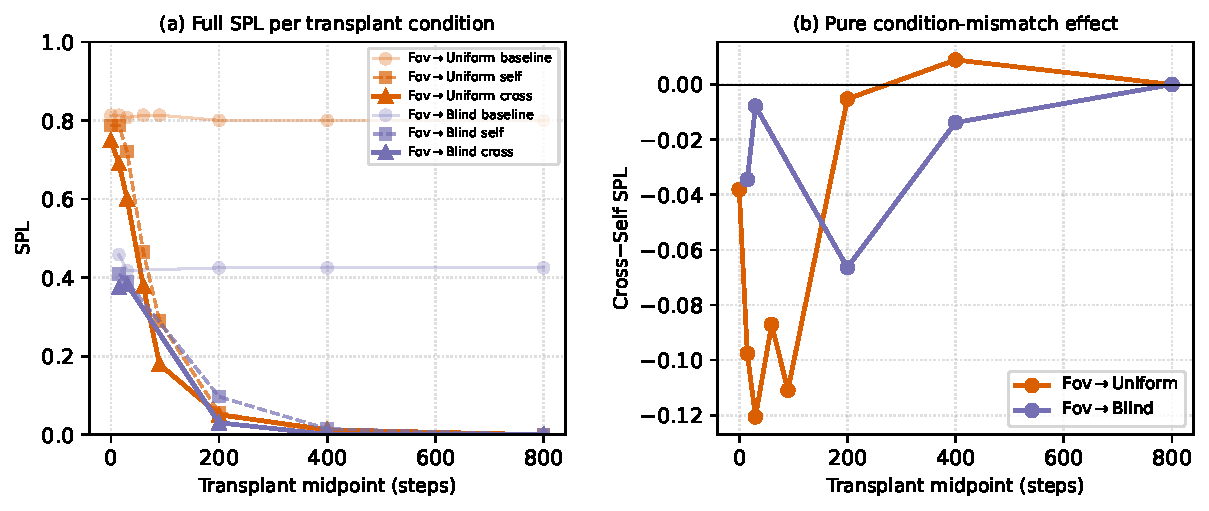
\includegraphics[width=0.95\linewidth]{fig/figa18_transplant_sweep.pdf}
\caption{\textbf{Memory-transplant midpoint sweep: the $t{=}30$ asymmetry is not a midpoint artefact.} Two representative donor$\to$recipient pairs (foveated$\to$uniform, foveated$\to$blind) across midpoints $\{0, 15, 30, 60, 90, 200, 400, 800\}$ time-steps ($n{=}100$--$150$ episodes/cell); the main-text $5{\times}5$ matrix is the $t{=}30$ slice. \textbf{(a)} Full SPL (baseline / self / cross): $t{=}0$ collapses to a protocol-noise floor (so the main-text diagonal reflects rollout divergence, not condition mismatch); for $t \geq 200$ all curves decay because most successful episodes have already terminated. \textbf{(b)} Cross$-$self isolates the pure condition-mismatch effect: it peaks at $t \in [30, 90]$ (the agent has integrated history but is not yet locked into a trajectory) and decays toward $0$ by $t \geq 400$.}
\label{fig:transplant_sweep_supp}
\end{figure}


\section{Encoder-Capacity Scaling: Log-Polar Foveation Control}
\label{app:scaling}

A direct test of the H1 mechanism (encoder spatial-feature variety per step drives top-layer LSTM spatial encoding) is to vary that variable continuously across our existing 4-condition spectrum. The most diagnostic single point is the \emph{log-polar foveation} control: log-polar resampling onto a $64{\times}64$ retinal grid produces an encoder spatial output of $\sim 2{\times}2$, intermediate between coarse's $1{\times}1$ and uniform's $4{\times}4$ (verified by direct forward pass through the trained encoder). Only the visual front-end differs from the foveated condition; LSTM, sensors, and training pipeline are identical. \textbf{Preregistered prediction:} if the H1 mechanism is the simple ``encoder spatial-output dimensionality'' reading, log-polar should produce LSTM GPS $R^2$ in the bottleneck regime (i.e.\ closer to coarse's $+0.58$ than to uniform's $\approx 0$); if log-polar matches uniform on H1 instead ($R^2 \approx 0$), the encoder-spatial-output mechanism story needs reframing toward channel information, encoder spatial-feature \emph{variety} per step, or another aspect. \textbf{Result (converged 250M frames).} The log-polar agent at convergence (ckpt-49, $\sim 245$M frames) yields top-layer GPS $R^2 = -0.029 \pm 0.759$ (5-fold CV, $n=500$ episodes) --- \emph{not} in the bottleneck regime, but indistinguishable from foveated ($R^2 = +0.178 \pm 0.659$) and clearly far from coarse ($R^2 = +0.582 \pm 0.099$). The simple ``encoder spatial-output dimensionality'' framing is therefore \emph{not} sufficient to explain the H1 phenomenon: log-polar's $2{\times}2$ output does not place it in the bottleneck regime. We read the result as supporting the alternative ``encoder spatial-feature \emph{variety} per step'' framing: log-polar's radial sampling preserves rich gaze-centred feature variety per timestep even at low spatial output, so the policy can still source position from the visual route and the LSTM does not commit capacity to the integrated code. Substitution-dynamics analysis (Figure~\ref{fig:magnitude}b) corroborates this reading: log-polar starts at $R^2 = +0.92$ at $\sim 50$M frames (matching all 4 main conditions' early high $R^2$), then decays along the rich-encoder trajectory rather than plateauing in the bottleneck range. A finer multi-point input-resolution sweep ($K \in \{32, 64, 96, 128, 192\}$) is reported as future work; its training cost (multiple from-scratch DD-PPO runs at $\sim 250$M frames each) was outside this submission's compute window.


\section{Architecture-Agnostic Confirmation: Memory Maze with DINOv2}
\label{app:wmprobe}

Companion figure to the architecture-agnostic claim in §\ref{sec:discussion}. Frozen DINOv2-Base patch features at five resolutions (matching our Habitat chassis: blind, coarse, foveated, uniform, log-polar) feed a small LSTM trained on Memory Maze $9{\times}9$ offline trajectories with a next-feature prediction objective; we then probe \texttt{agent\_pos} from the LSTM hidden state (Ridge linear and 4-layer MLP probes, frame-level $80/20$ split, eval window steps $250$--$500$ of $T{=}500$ trajectories).

\begin{figure}[!t]
  \centering
  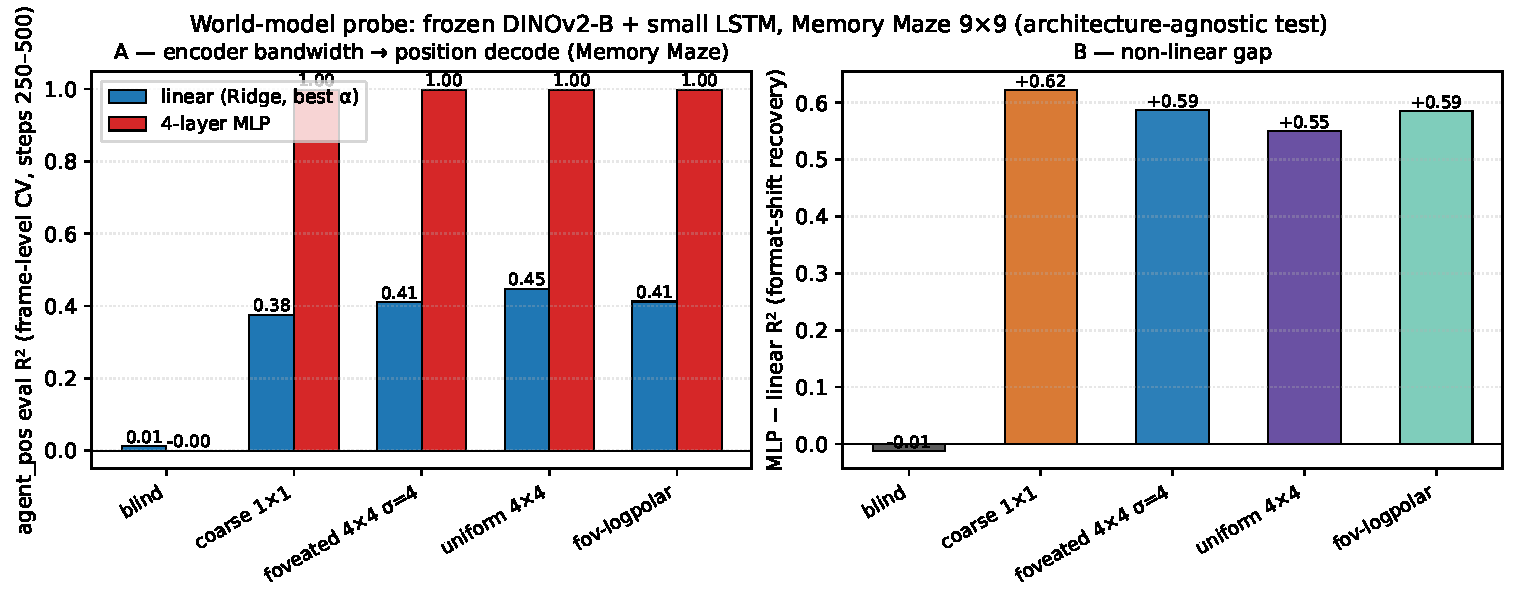
\includegraphics[width=\linewidth]{fig/fig9_world_model_probe.pdf}
  \caption{\textbf{Format shift reproduces on Memory Maze with a frozen DINOv2-Base encoder.} \emph{(a)} Linear (Ridge, blue) and 4-layer MLP (red) eval $R^2$ for \texttt{agent\_pos} from the LSTM hidden state. Linear $R^2$ rises with encoder bandwidth (blind $0.01 \to$ uniform $0.45$); MLP $R^2$ saturates at $\approx 0.998$ for all sighted conditions and stays at chance for blind. \emph{(b)} Non-linear gap (MLP$-$linear) decreases with bandwidth (coarse $+0.62$ vs.\ uniform $+0.55$): the same format-shift dichotomy as Habitat. The reversed linear-$R^2$ direction across the bandwidth axis reflects Memory Maze's lack of GPS/compass channels: the encoder is the only sensory route to absolute position, so blind carries no signal at all.}
  \label{fig:wmprobe}
\end{figure}


\end{document}
